\documentclass[12pt]{article}

\usepackage{babel}
\usepackage[utf8]{inputenc}
\usepackage[T1]{fontenc}
\usepackage{mathpazo}
\usepackage{microtype}
\usepackage{stmaryrd}
\usepackage{amsmath,amssymb,amsthm}
\usepackage{mathtools}
\usepackage{geometry}
\usepackage{hyperref}
\usepackage{tikz}
\usepackage{tikz-cd}
\usepackage{pgfplots}
\usepackage{csquotes}
\usepackage{setspace}
\usepackage{fancyhdr}
\usepackage{xcolor}
\usepackage{mdframed}
\usepackage{caption}
\usepackage{subcaption}

\usetikzlibrary{arrows,arrows.meta,positioning,shapes,shapes.geometric,fit,calc,
                decorations.pathmorphing,decorations.markings,backgrounds,
                matrix,chains,scopes,hobby,patterns}
\pgfplotsset{compat=1.18}

\geometry{margin=1in, top=1.2in, bottom=1.2in}
\setstretch{1.15}

\pagestyle{fancy}
\fancyhf{}
\fancyhead[L]{\small\textit{Introducción a Spherepop}}
\fancyhead[R]{\small\thepage}
\renewcommand{\headrulewidth}{0.4pt}

\theoremstyle{plain}
\newtheorem{theorem}{Teorema}[section]
\newtheorem{proposition}[theorem]{Proposición}
\newtheorem{lemma}[theorem]{Lema}
\newtheorem{corollary}[theorem]{Corolario}

\theoremstyle{definition}
\newtheorem{definition}[theorem]{Definición}
\newtheorem{example}[theorem]{Ejemplo}
\newtheorem{remark}[theorem]{Observación}
\newtheorem{axiom}[theorem]{Axioma}

\colorlet{bubbleblue}{blue!12}
\colorlet{bubbleteal}{teal!15}
\colorlet{bubblegray}{gray!10}
\colorlet{arrowcolor}{black!70}

\title{Introducción a Spherepop\\
\large Un cálculo de historia de eventos}
\author{Flyxion}
\date{\today}

\begin{document}

\maketitle
\thispagestyle{empty}

\begin{abstract}
\footnotesize
\noindent
Este ensayo introduce \emph{Spherepop}, un marco conceptual, visual y formal basado en eventos irreversibles para la construcción de significado, identidad y computación. A diferencia de los sistemas matemáticos y computacionales que parten de estados, conjuntos o axiomas atemporales~\cite{barendregt,homotopy}, Spherepop comienza con eventos que ocurren una sola vez, modifican el espacio de posibilidades posteriores y dejan un historial auditable. Bajo esta perspectiva, la estructura no se supone previamente dada sino que emerge de la acumulación histórica de acciones, en un sentido análogo al que Whitehead denomina el carácter ``processual'' de la realidad~\cite{whitehead}.

El enfoque propone una mereología constructiva basada en la historia~\cite{simons}, donde las relaciones parte-todo se forman gradualmente conforme ocurren eventos que integran nuevos componentes en estructuras existentes. La identidad de los objetos no se define por pertenencia abstracta ni por propiedades intrínsecas aisladas, sino por el historial de eventos que los ha producido, en consonancia con el principio de individuación causal discutido por Kim~\cite{kim} y Fine~\cite{fine}. Dos entidades se consideran idénticas si y sólo si comparten exactamente el mismo historial de eventos que les dio origen.

Spherepop se presenta también como un lenguaje visual de ámbitos anidados representados por burbujas evaluadas explícitamente, que hace visibles relaciones frecuentemente implícitas en otros sistemas formales~\cite{girard,abramsky}, como el alcance, el orden de evaluación y las dependencias históricas entre eventos. Su formalización matemática se articula dentro de la teoría de categorías~\cite{maclane,awodey}, donde los eventos actúan como morfismos irreversibles que transforman espacios de opciones. Se demuestra que el sistema resultante es expresivamente equivalente a sistemas computacionales concatenativos completos~\cite{moore} y se conecta con trabajos sobre irreversibilidad y entropía computacional~\cite{landauer,bennett}. El ensayo desarrolla estas ideas mediante ejemplos cotidianos y formalizaciones matemáticas que muestran cómo estructuras complejas pueden surgir de la acumulación de eventos históricos sin recurrir a pertenencia global ni a comprensión irrestricta.
\end{abstract}

\newpage
\tableofcontents
\newpage

\section{Introducción}
\label{sec:intro}

La mayor parte de los lenguajes formales con los que se describen la lógica, la matemática y la computación comienza con entidades que ya se suponen disponibles. En la tradición cantoniana se parte de conjuntos y relaciones de pertenencia~\cite{cantor,zermelo}; en los sistemas de tipos se parte de tipos habitados y funciones entre ellos~\cite{martinlof,homotopy}; en los sistemas operacionales de la semántica denotacional se parte de dominios ya construidos~\cite{scottdana,abramsky}. Incluso cuando estos sistemas permiten describir cambio, ejecución o transformación, con frecuencia lo hacen sobre un fondo conceptual donde la estructura básica ya estaba disponible antes de cualquier acontecimiento. El presente ensayo propone invertir ese orden de fundamentación.

\emph{Spherepop} parte de la hipótesis de que la historia no es un accidente secundario de los sistemas reales, sino su condición constitutiva. Antes que estados estáticos o totalidades dadas de antemano, lo primero son eventos irreversibles. Un evento irreversible es una ocurrencia que no sólo sucede, sino que altera el espacio de posibilidades posteriores y deja un rastro. Una vez ocurrido, el sistema ya no se encuentra conceptualmente en la misma situación que antes. La estructura, bajo esta perspectiva, no es originaria sino sedimentada. Esta orientación tiene antecedentes filosóficos en la ontología del proceso de Whitehead~\cite{whitehead}, en la fenomenología de la temporalidad de Heidegger~\cite{heidegger}, y en la filosofía del acontecimiento de Badiou~\cite{badiou}, aunque el presente trabajo no persigue una exégesis de ninguna de estas tradiciones sino la construcción de un aparato formal original.

Esta intuición se vuelve inmediata en ejemplos cotidianos. Cuando una persona envía un mensaje, no sólo produce una cadena de texto sino que crea una nueva situación interpersonal con consecuencias posibles que antes no existían: una respuesta, un malentendido, una reconciliación o un conflicto. Del mismo modo, cuando una taza se rompe no estamos frente a una simple transición entre dos estados equivalentes de una descripción física, sino ante una irreversibilidad concreta que reorganiza las acciones disponibles~\cite{prigogine}. Ambos ejemplos comparten una estructura formal: el evento modifica el horizonte de acciones futuras de manera que no puede revertirse sin introducir nuevos eventos que reconfiguren el sistema.

Spherepop toma en serio este tipo de ejemplos y los eleva al rango de principio formal. En lugar de preguntar primero qué objetos existen y después cómo interactúan, pregunta qué eventos han ocurrido y qué estructuras han quedado constituidas por ellos. El cambio de punto de partida es profundo. Significa que la identidad de una entidad no se entiende como una esencia previa~\cite{aristoteles} sino como una trayectoria histórica~\cite{kim}. También significa que las relaciones parte-todo no se conciben como mera inclusión abstracta entre elementos ya definidos, sino como articulaciones que se construyen a través de secuencias de incorporación, dependencia y estabilización~\cite{simons,varzi}.

Esta orientación responde además a una dificultad recurrente en múltiples tradiciones formales. Cuando se parte de mecanismos de pertenencia global o de principios de comprensión demasiado amplios, aparecen paradojas y sobrecargas ontológicas bien documentadas~\cite{russellparadox,zermelo}. La tentación de definir cualquier colección por cualquier propiedad genera sistemas poderosos pero también ambigüedades y tensiones conceptuales difíciles de resolver. Spherepop propone un camino distinto: en lugar de permitir que la complejidad crezca por licencia axiomática, restringe su crecimiento a lo que efectivamente ha sucedido. Sólo hay estructura allí donde ha habido historia. Sólo hay identidad allí donde puede trazarse una continuidad de eventos. Sólo hay composición allí donde una relación constructiva la ha producido.

Bajo esta formulación, el lenguaje visual de las burbujas no es un adorno pedagógico sino una consecuencia natural del marco. Si las dependencias, los ámbitos y las evaluaciones son históricas, entonces conviene representarlas de manera en que el alcance y la anidación sean visibles. Las burbujas de Spherepop cumplen precisamente esa función: hacen perceptible que ciertos procesos ocurren dentro de otros, que ciertas evaluaciones sólo tienen sentido en contextos delimitados, y que la forma en que una estructura se integra a otra depende del orden concreto en que los eventos han tenido lugar. La Figura~\ref{fig:burbujas_intro} ofrece una primera ilustración de este principio.

\begin{figure}[ht]
\centering
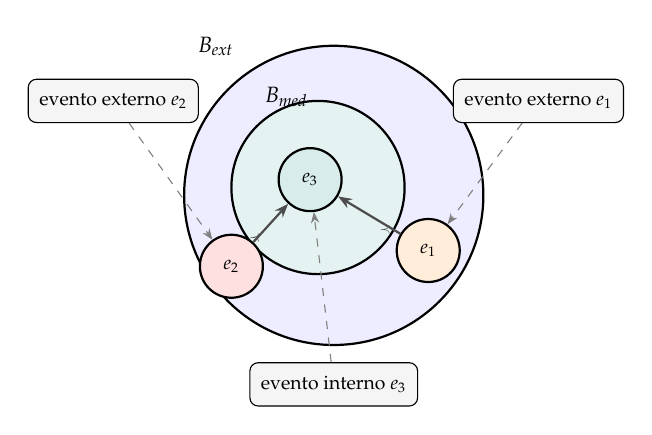
\begin{tikzpicture}[
  bubble/.style={circle, draw, thick, fill=bubbleblue, minimum size=1.2cm, font=\small},
  innerbubble/.style={circle, draw, thick, fill=bubbleteal, minimum size=0.8cm, font=\scriptsize},
  event/.style={rectangle, draw, rounded corners=3pt, fill=gray!8, minimum height=0.55cm,
                font=\scriptsize, inner sep=4pt},
  arr/.style={-{Stealth[length=5pt]}, thick, color=arrowcolor}
]

\node[bubble, minimum size=3.8cm, fill=blue!7] (outer) at (0,0) {};
\node[anchor=south west, font=\footnotesize\itshape] at (-1.85,1.65) {$B_{\text{ext}}$};

\node[bubble, minimum size=2.2cm, fill=teal!10] (mid) at (-0.2, 0.1) {};
\node[anchor=south west, font=\footnotesize\itshape] at (-1.0, 1.0) {$B_{\text{med}}$};

\node[innerbubble] (inner) at (-0.3, 0.2) {$e_3$};
\node[innerbubble, fill=orange!15] (e1) at (1.2, -0.7) {$e_1$};
\node[innerbubble, fill=red!12] (e2) at (-1.3, -0.9) {$e_2$};

\draw[arr] (e1) -- (inner) node[midway, below right, font=\tiny] {$\prec$};
\draw[arr] (e2) -- (inner) node[midway, below left, font=\tiny] {$\prec$};

\node[event] (lab1) at (2.6, 1.2) {evento externo $e_1$};
\node[event] (lab2) at (-2.8, 1.2) {evento externo $e_2$};
\node[event] (lab3) at (0, -2.4) {evento interno $e_3$};

\draw[-{Stealth[length=4pt]}, dashed, gray] (lab1) -- (e1);
\draw[-{Stealth[length=4pt]}, dashed, gray] (lab2) -- (e2);
\draw[-{Stealth[length=4pt]}, dashed, gray] (lab3) -- (inner);
\end{tikzpicture}
\caption{Representación introductoria de ámbitos anidados en Spherepop. La burbuja exterior $B_{\text{ext}}$ contiene a $B_{\text{med}}$, cuyo interior aloja el evento $e_3$. Los eventos externos $e_1$ y $e_2$ preceden causalmente a $e_3$, representado por las flechas de precedencia $\prec$.}
\label{fig:burbujas_intro}
\end{figure}

El objetivo de este ensayo es exponer la propuesta en un recorrido gradual. En la Sección~\ref{sec:motivacion} se introducen intuiciones básicas a partir de experiencias ordinarias. La Sección~\ref{sec:mereologia} desarrolla la mereología histórica. La Sección~\ref{sec:identidad} formaliza la identidad como historial compartido. La Sección~\ref{sec:ambitos} introduce los ámbitos anidados y su representación visual. La Sección~\ref{sec:previo} sitúa el trabajo en relación con tradiciones existentes. Las Secciones~\ref{sec:formalizacion} a~\ref{sec:maquina} desarrollan la formalización matemática progresivamente. Las secciones finales discuten las implicaciones para sistemas reales y concluyen el trabajo. Los apéndices presentan material técnico adicional.

Desde esta perspectiva, Spherepop puede leerse simultáneamente como filosofía de la estructura, como lenguaje visual y como programa formal. Su apuesta central consiste en afirmar que significado, identidad y computación no deben derivarse de entidades estáticas a las que después se añade el tiempo, sino de eventos situados cuyo carácter irreversible constituye la trama misma de lo real formalizable.

\section{Motivación: comenzar con eventos en lugar de estados}
\label{sec:motivacion}

La motivación principal de Spherepop surge de una insatisfacción con los marcos descriptivos que tratan el cambio como una modificación externa de estructuras ya completas. En muchos modelos de la semántica de programas~\cite{abramsky,plotkin}, un sistema se representa como una colección de estados posibles y una relación de transición entre ellos. Esta estrategia tiene utilidad indudable, pero encierra una presuposición fuerte: lo fundamental sería el espacio de estados, mientras que la historia concreta de las transiciones sería secundaria, o en el mejor de los casos derivable. Spherepop invierte esa prioridad y propone que la historia efectiva es anterior, tanto conceptual como constructivamente, al inventario abstracto de estados.

La diferencia se aprecia con claridad en situaciones ordinarias. Considérese el acto de firmar un contrato. Desde una perspectiva puramente estática podría decirse que antes existía un estado en que el contrato no estaba firmado y después otro en que sí lo estaba. Sin embargo, esa descripción pierde el núcleo de la situación. Lo decisivo no es sólo que el sistema haya cambiado de un estado a otro, sino que ocurrió un acto fechado, situado y vinculante que reconfiguró derechos, expectativas y obligaciones~\cite{searle,austin}. Lo que importa no es sólo la fotografía del antes y del después, sino el hecho de que un evento ocurrió y dejó consecuencias normativas. La firma no es un detalle accidental de la transición; es el origen histórico de una nueva estructura institucional.

Algo semejante ocurre al guardar un archivo con cambios importantes. Después de escribir un párrafo nuevo o borrar una sección entera, el documento puede todavía llevar el mismo nombre. Sin embargo, su identidad operativa ha cambiado porque existe una secuencia concreta de ediciones que explica por qué ese archivo es ahora lo que es~\cite{chacon}. El documento no se comprende adecuadamente si se lo trata como un estado aislado; se comprende mejor como la condensación de una historia de modificaciones donde cada guardado delimita un umbral, cada revisión agrega irreversibilidad, y aun cuando el sistema permite deshacer ciertas acciones, esa capacidad misma depende de haber conservado el historial de los pasos previos~\cite{okasaki}.

La vida social ofrece ejemplos todavía más inmediatos. Una amistad no consiste en un conjunto abstracto de propiedades compartidas entre dos personas, sino en una secuencia de encuentros, conversaciones, favores, tensiones y recuerdos~\cite{goffman}. Cuando alguien recuerda una discusión, una promesa o una traición, no está introduciendo detalles contingentes a una identidad ya definida; está señalando los eventos que constituyen esa identidad relacional. La historia no se agrega desde fuera; es el medio mismo de individuación~\cite{kim,fine}.

Spherepop generaliza esta observación. Un sistema real, sea cognitivo, computacional o social, no se distingue solamente por las configuraciones que pueden describirse en un instante, sino por la secuencia irreversible de eventos que lo ha llevado hasta allí. Esto obliga a revisar el punto de partida de la formalización. Si la historia es constitutiva, entonces no conviene modelar primero un universo de objetos ya delimitados para después introducir cambios. Conviene modelar eventos, rastros y dependencias, y dejar que de ahí emerjan los objetos y sus relaciones~\cite{winskel,pratt}.

Esta prioridad de los eventos también tiene una ventaja de economía conceptual. En los sistemas basados en estados, suele ser necesario postular un espacio muy amplio de posibilidades para alojar todas las configuraciones concebibles. En cambio, un enfoque histórico permite que la complejidad crezca únicamente a partir de lo que efectivamente ocurre. No es necesario suponer de entrada una totalidad exuberante de entidades posibles; basta con registrar qué ha sucedido, qué ha quedado fijado por ello y qué nuevas posibilidades se han abierto o cerrado como consecuencia~\cite{fowler,eventcollaborator}.

Por esa razón, Spherepop no entiende los eventos como meras actualizaciones sobre una base previamente establecida. Cada evento es una operación constitutiva que introduce una diferencia duradera, deja una marca y modifica las condiciones de integración de eventos futuros. La tesis puede formularse de manera precisa: un sistema no debe definirse primariamente por lo que contiene en abstracto, sino por lo que le ha ocurrido. La pregunta fundamental deja de ser ``¿qué elementos pertenecen aquí?'' y pasa a ser ``¿qué eventos han constituido este aquí?''. Esta reformulación no sólo cambia la semántica del sistema; cambia también su lógica de construcción, su noción de identidad y su manera de visualizar el alcance, la dependencia y el orden.

\section{Mereología histórica y construcción de estructura}
\label{sec:mereologia}

Si los eventos irreversibles constituyen el punto de partida de Spherepop, entonces las relaciones parte-todo no pueden entenderse como inclusión abstracta entre elementos previamente dados. En cambio, deben concebirse como el resultado de una historia de incorporación. La mereología~\cite{simons,varzi,casati}, bajo este enfoque, no describe simplemente cómo se organizan entidades ya existentes, sino cómo ciertas entidades llegan a formar parte de otras a través de eventos concretos.

Para ilustrar esta idea conviene considerar un ejemplo cotidiano. Supóngase la construcción de una casa. La casa no aparece como una totalidad completa desde el principio. Primero se delimita un terreno, después se colocan los cimientos, posteriormente se levantan las paredes, se instala el techo y se añaden puertas, ventanas y sistemas internos. Cada paso es un evento que modifica la estructura existente. Cuando una pared se integra a los cimientos, la relación parte-todo no es una relación lógica abstracta; es la consecuencia histórica de un acto constructivo específico~\cite{simons}.

\begin{figure}[ht]
\centering
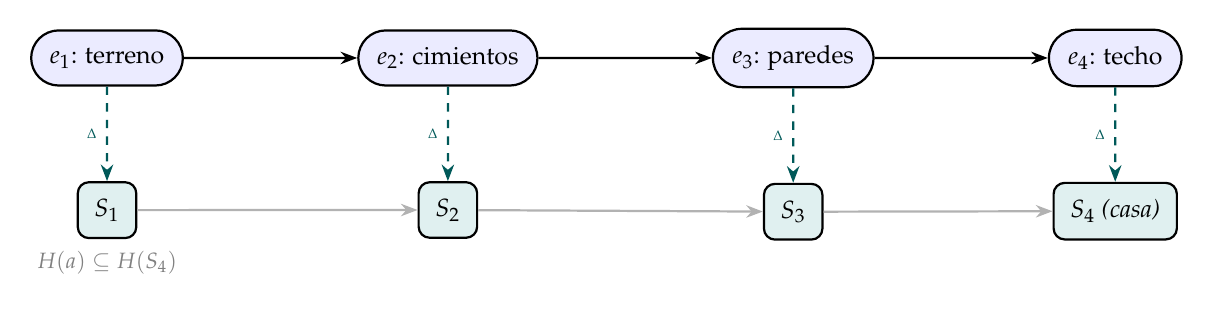
\begin{tikzpicture}[
  node distance=1.5cm and 2.2cm,
  ev/.style={rounded rectangle, draw, thick, fill=blue!8, minimum height=0.7cm,
             font=\small, inner sep=6pt},
  str/.style={rectangle, draw, thick, fill=teal!12, rounded corners=4pt,
              minimum height=0.7cm, font=\small\itshape, inner sep=6pt},
  arr/.style={-{Stealth[length=6pt]}, thick},
  inc/.style={-{Stealth[length=6pt]}, thick, dashed, teal!70!black}
]
\node[ev] (e1) {$e_1$: terreno};
\node[ev, right=of e1] (e2) {$e_2$: cimientos};
\node[ev, right=of e2] (e3) {$e_3$: paredes};
\node[ev, right=of e3] (e4) {$e_4$: techo};

\node[str, below=1.2cm of e1] (s1) {$S_1$};
\node[str, below=1.2cm of e2] (s2) {$S_2$};
\node[str, below=1.2cm of e3] (s3) {$S_3$};
\node[str, below=1.2cm of e4] (s4) {$S_4$ (casa)};

\draw[arr] (e1) -- (e2);
\draw[arr] (e2) -- (e3);
\draw[arr] (e3) -- (e4);

\draw[inc] (e1) -- (s1) node[midway, left, font=\tiny] {$\Delta$};
\draw[inc] (e2) -- (s2) node[midway, left, font=\tiny] {$\Delta$};
\draw[inc] (e3) -- (s3) node[midway, left, font=\tiny] {$\Delta$};
\draw[inc] (e4) -- (s4) node[midway, left, font=\tiny] {$\Delta$};

\draw[arr, gray!60] (s1) -- (s2);
\draw[arr, gray!60] (s2) -- (s3);
\draw[arr, gray!60] (s3) -- (s4);

\node[font=\footnotesize\itshape, gray] at (0, -2.6) {$H(a) \subseteq H(S_4)$};
\end{tikzpicture}
\caption{Mereología histórica de la construcción de una casa. Cada evento $e_i$ contribuye con un incremento estructural $\Delta(e_i)$ que expande la estructura $S_i$ en $S_{i+1}$. La relación parte-todo se deriva de la inclusión de historiales: $H(\text{cimientos}) \subseteq H(\text{casa})$.}
\label{fig:mereologia}
\end{figure}

Un fenómeno semejante ocurre en el ámbito digital. Cuando un programador desarrolla un proyecto de software, el repositorio no es una colección estática de archivos; se forma mediante una serie de confirmaciones, modificaciones y revisiones~\cite{chacon}. Cada confirmación incorpora cambios específicos y establece una nueva versión del sistema. Un archivo forma parte del proyecto porque ha sido añadido o modificado en un evento histórico particular dentro del repositorio. Incluso si dos archivos tienen el mismo contenido, su papel dentro del proyecto depende del historial que los vincula con ese sistema de desarrollo.

Spherepop generaliza esta intuición mediante una mereología basada en eventos. Las relaciones parte-todo se establecen cuando ocurre un evento de incorporación, el cual registra que una estructura existente se ha expandido para incluir un nuevo componente.

\begin{definition}[Historia de eventos]
\label{def:historia}
Sea $E$ un conjunto de eventos irreversibles. Una \emph{historia} es un par ordenado $H = (E_H, \prec)$ donde $E_H \subseteq E$ es el conjunto de eventos que han ocurrido y $\prec$ es una relación de orden parcial estricto sobre $E_H$ que representa la precedencia causal. La relación $\prec$ satisface:
\[
\text{irreflexividad:}\quad \neg(e \prec e), \qquad
\text{transitividad:}\quad e_1 \prec e_2 \land e_2 \prec e_3 \Rightarrow e_1 \prec e_3.
\]
\end{definition}

\begin{definition}[Función de incremento estructural]
\label{def:delta}
Para cada evento $e \in E_H$ se define una \emph{función de contribución estructural} $\Delta(e)$ que representa la modificación introducida por $e$ en la estructura del sistema. La estructura en el estado $t$ es
\[
S_t = \bigsqcup_{e \in E_H,\, e \prec t} \Delta(e)
\]
donde $\bigsqcup$ denota la amalgamación histórica de contribuciones, respetando las dependencias causales.
\end{definition}

\begin{definition}[Mereología histórica]
\label{def:mereologia}
Una entidad $a$ es \emph{parte mereológica histórica} de una entidad $b$, escrito $a \preceq_M b$, si y sólo si el historial que constituye $a$ está contenido en el historial que constituye $b$:
\[
a \preceq_M b \quad\Longleftrightarrow\quad H(a) \subseteq H(b),
\]
donde $H(x)$ denota el conjunto de eventos que han contribuido a la formación de la entidad $x$.
\end{definition}

\begin{proposition}
\label{prop:mereologia_preorden}
La relación $\preceq_M$ es un preorden sobre el conjunto de entidades del sistema, y es un orden parcial si la relación de historial es antisimétrica.
\end{proposition}

\begin{proof}
La reflexividad $a \preceq_M a$ se sigue inmediatamente de $H(a) \subseteq H(a)$. La transitividad: si $H(a) \subseteq H(b)$ y $H(b) \subseteq H(c)$ entonces $H(a) \subseteq H(c)$, de donde $a \preceq_M c$. La antisimetría: si $H(a) \subseteq H(b)$ y $H(b) \subseteq H(a)$ entonces $H(a) = H(b)$, lo cual define la identidad histórica en la Definición~\ref{def:identidad} de la sección siguiente.
\end{proof}

Esta reformulación tiene consecuencias importantes. En primer lugar, elimina la necesidad de postular un universo global de pertenencia donde todas las relaciones posibles estén definidas desde el inicio~\cite{zermelo}. En segundo lugar, garantiza que la complejidad del sistema crezca únicamente en función de los eventos que realmente han ocurrido. Finalmente, permite que la estructura del sistema refleje de manera directa la historia de su formación~\cite{simons,fowler}.

\section{Identidad como historial de eventos}
\label{sec:identidad}

Si la estructura de un sistema emerge de la acumulación de eventos irreversibles, entonces la identidad de sus componentes tampoco puede entenderse como una propiedad previa e independiente de la historia. En Spherepop, la identidad es el resultado de una trayectoria histórica~\cite{kim,fine,wiggins}. Dos entidades son idénticas si y sólo si comparten exactamente el mismo historial de eventos que las ha producido.

Esta idea puede parecer inusual en términos formales, pero en la vida cotidiana resulta bastante natural. Considérese el caso de un documento digital. Dos archivos pueden contener exactamente el mismo texto en un momento dado y, sin embargo, si uno fue escrito directamente y el otro es una copia creada posteriormente, su historia es diferente. En muchos contextos esa diferencia importa: un documento original firmado tiene un valor jurídico distinto al de una copia, incluso si el contenido textual es idéntico~\cite{austin}. Lo que distingue al original no es su estructura visible, sino la secuencia de eventos que lo produjo.

Algo similar ocurre con la identidad personal en la tradición filosófica anglosajona~\cite{parfit,locke}. Dos individuos pueden compartir características físicas o psicológicas similares, pero su identidad no depende únicamente de esas propiedades; depende de la historia de eventos que han vivido. En este sentido, la identidad se comporta más como una trayectoria que como una etiqueta.

\begin{definition}[Historial de una entidad]
\label{def:historial}
Sea $x$ una entidad dentro de un sistema con historia $H = (E_H, \prec)$. El \emph{historial de $x$} es el conjunto
\[
H(x) = \bigl\{ e \in E_H \mid e \text{ contribuye causalmente a la formación de } x \bigr\}.
\]
Este conjunto hereda la relación de precedencia causal de $H$, de modo que $(H(x), \prec|_{H(x)})$ es a su vez un orden parcial estricto.
\end{definition}

\begin{definition}[Identidad histórica]
\label{def:identidad}
Dos entidades $x$ e $y$ son \emph{históricamente idénticas}, escrito $x =_H y$, si y sólo si sus historiales coinciden:
\[
x =_H y \quad\Longleftrightarrow\quad H(x) = H(y).
\]
\end{definition}

\begin{remark}
La identidad histórica es más fina que la igualdad observacional. Dos entidades pueden ser observacionalmente indistinguibles en un momento dado, es decir, compartir todos sus atributos presentes, y sin embargo tener historiales distintos. La Definición~\ref{def:identidad} las trataría como entidades distintas, reflejando así diferencias causales que podrían ser relevantes para el comportamiento futuro del sistema~\cite{kim,fine}. Esta distinción es análoga a la que Parfit realiza entre continuidad psicológica e identidad personal~\cite{parfit}.
\end{remark}

La Figura~\ref{fig:identidad} ilustra el contraste entre identidad observacional e identidad histórica mediante un diagrama de divergencia de historiales.

\begin{figure}[ht]
\centering
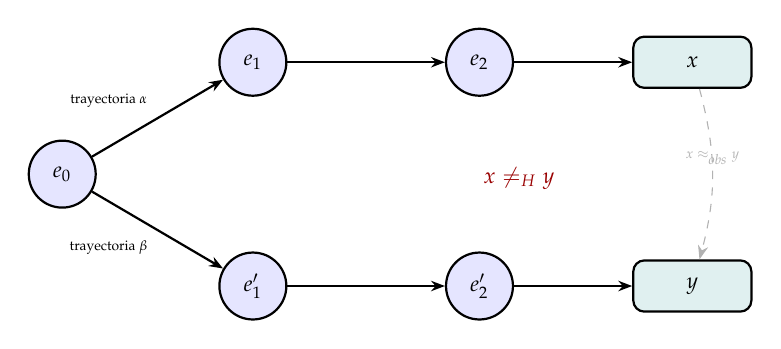
\begin{tikzpicture}[
  node distance=1.2cm and 1.8cm,
  ev/.style={circle, draw, thick, fill=blue!10, minimum size=0.85cm, font=\footnotesize},
  ob/.style={rectangle, draw, thick, fill=teal!12, rounded corners=4pt,
             minimum height=0.65cm, minimum width=1.5cm, font=\footnotesize},
  arr/.style={-{Stealth[length=5pt]}, thick},
  dashed arr/.style={-{Stealth[length=5pt]}, dashed, gray!60}
]
\node[ev] (e0) {$e_0$};
\node[ev, above right=0.8cm and 1.8cm of e0] (e1a) {$e_1$};
\node[ev, below right=0.8cm and 1.8cm of e0] (e1b) {$e_1'$};
\node[ev, right=2cm of e1a] (e2a) {$e_2$};
\node[ev, right=2cm of e1b] (e2b) {$e_2'$};
\node[ob, right=1.5cm of e2a] (xa) {$x$};
\node[ob, right=1.5cm of e2b] (xb) {$y$};

\draw[arr] (e0) -- (e1a) node[midway, above left, font=\tiny] {trayectoria $\alpha$};
\draw[arr] (e0) -- (e1b) node[midway, below left, font=\tiny] {trayectoria $\beta$};
\draw[arr] (e1a) -- (e2a);
\draw[arr] (e1b) -- (e2b);
\draw[arr] (e2a) -- (xa);
\draw[arr] (e2b) -- (xb);

\draw[dashed arr, bend left=15] (xa) to node[above, font=\tiny\itshape] {$x \approx_{\text{obs}} y$} (xb);
\node[font=\footnotesize\itshape, red!60!black] at (5.8, -0.05) {$x \neq_H y$};

\end{tikzpicture}
\caption{Divergencia entre identidad observacional e identidad histórica. Dos entidades $x$ e $y$ pueden ser observacionalmente similares ($x \approx_{\text{obs}} y$) pero históricamente distintas ($x \neq_H y$) cuando sus historiales divergen a partir de un punto común $e_0$.}
\label{fig:identidad}
\end{figure}

Desde un punto de vista computacional, la identidad basada en historial tiene implicaciones concretas. En sistemas distribuidos, la consistencia de los datos depende a menudo de mantener un registro ordenado de operaciones que han ocurrido en el sistema~\cite{lamport,shapiro}. Técnicas como los registros de eventos o las cadenas de bloques funcionan precisamente porque cada estado se deriva de una secuencia verificable de eventos anteriores~\cite{kleppmann,nakamoto}. Spherepop generaliza este principio y lo convierte en una definición fundamental de identidad.

\begin{theorem}[Conservación de la identidad bajo extensión compatible]
\label{thm:conservacion}
Sea $H = (E_H, \prec)$ una historia y sean $x, y$ dos entidades con $x =_H y$. Si se añade un nuevo evento $e \notin E_H$ que contribuye a ambas de la misma manera, la identidad se conserva: $x =_{H'} y$ en la historia extendida $H' = (E_H \cup \{e\}, \prec')$.
\end{theorem}

\begin{proof}
Por hipótesis $H(x) = H(y)$. El nuevo evento $e$ contribuye a la formación de $x$ si y sólo si contribuye a la formación de $y$, por la condición de compatibilidad. Por lo tanto $H'(x) = H(x) \cup \{e\} = H(y) \cup \{e\} = H'(y)$, lo que da $x =_{H'} y$.
\end{proof}

\section{Ámbitos anidados y representación visual mediante burbujas}
\label{sec:ambitos}

Una consecuencia importante del enfoque histórico de Spherepop es que el alcance, la dependencia y el orden de evaluación dejan de ser aspectos implícitos del sistema y pasan a ser propiedades visibles de su estructura. Si los eventos se organizan históricamente y si las relaciones parte-todo surgen de incorporaciones sucesivas, entonces resulta natural representar estas relaciones mediante ámbitos anidados~\cite{church,plotkin}. En Spherepop estos ámbitos se visualizan mediante burbujas.

La idea básica puede entenderse a partir de situaciones cotidianas donde los contextos se encuentran contenidos unos dentro de otros. Considérese una conversación en una reunión: dentro de una reunión general pueden surgir pequeños grupos de discusión, y dentro de uno de esos grupos alguien puede contar una historia que incluye otra conversación anterior. Cada nivel introduce un nuevo contexto que delimita qué afirmaciones tienen sentido en ese momento~\cite{goffman,austin}. Lo que se dice dentro de una historia no necesariamente se aplica al contexto de la reunión completa. El significado depende del ámbito en que se produce el evento lingüístico.

\begin{definition}[Burbuja y ámbito histórico]
\label{def:burbuja}
Una \emph{burbuja} $B$ es un par $(E_B, \prec_B)$ donde $E_B \subseteq E_H$ es un subconjunto de eventos y $\prec_B = \prec|_{E_B}$ es la restricción de la precedencia causal a ese subconjunto. La \emph{relación de anidación} entre burbujas se define como:
\[
B_1 \subseteq_{\mathcal{B}} B_2 \quad\Longleftrightarrow\quad E_{B_1} \subseteq E_{B_2}.
\]
Un evento $e \in E_B$ se dice \emph{propio} de $B$ si $e \notin E_{B'}$ para ninguna sub-burbuja $B' \subsetneq_{\mathcal{B}} B$.
\end{definition}

\begin{remark}
En términos computacionales, la estructura de burbujas es análoga al concepto de alcance léxico en lenguajes de programación~\cite{church,plotkin}. Una función puede definir variables locales cuyo significado depende del bloque de código en que aparecen. Sin embargo, en Spherepop la noción de alcance no se limita a un mecanismo sintáctico; se vincula directamente con la historia de los eventos que han construido ese ámbito~\cite{winskel}.
\end{remark}

La Figura~\ref{fig:burbujas_anidadas} ilustra una jerarquía de burbujas con eventos distribuidos en distintos niveles de alcance.

\begin{figure}[ht]
\centering
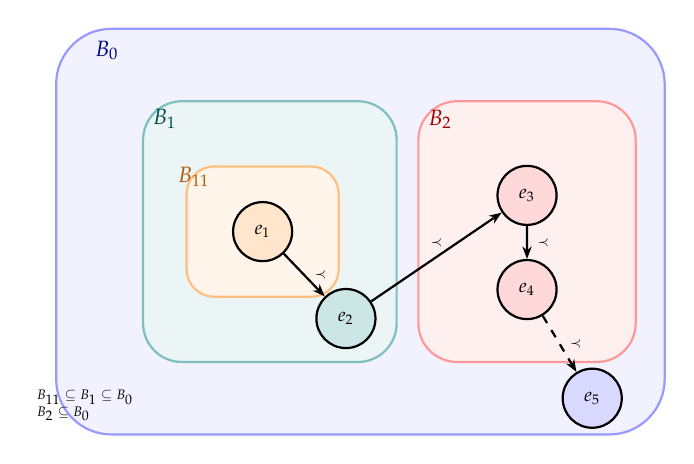
\begin{tikzpicture}[scale=0.92]
\begin{scope}
  \filldraw[fill=blue!5, draw=blue!40, thick, rounded corners=20pt]
    (-4.2,-2.8) rectangle (4.2,2.8);
  \node[font=\footnotesize\itshape, blue!50!black] at (-3.5, 2.5) {$B_0$};
\end{scope}
\begin{scope}
  \filldraw[fill=teal!8, draw=teal!50, thick, rounded corners=14pt]
    (-3.0,-1.8) rectangle (0.5,1.8);
  \node[font=\footnotesize\itshape, teal!60!black] at (-2.7, 1.55) {$B_1$};
\end{scope}
\begin{scope}
  \filldraw[fill=orange!8, draw=orange!50, thick, rounded corners=10pt]
    (-2.4,-0.9) rectangle (-0.3,0.9);
  \node[font=\footnotesize\itshape, orange!70!black] at (-2.3, 0.75) {$B_{11}$};
\end{scope}
\begin{scope}
  \filldraw[fill=red!6, draw=red!40, thick, rounded corners=14pt]
    (0.8,-1.8) rectangle (3.8,1.8);
  \node[font=\footnotesize\itshape, red!60!black] at (1.1, 1.55) {$B_2$};
\end{scope}

\node[circle, draw, fill=orange!20, thick, minimum size=0.75cm, font=\scriptsize]
  (e1) at (-1.35, 0) {$e_1$};
\node[circle, draw, fill=teal!20, thick, minimum size=0.75cm, font=\scriptsize]
  (e2) at (-0.2, -1.2) {$e_2$};
\node[circle, draw, fill=red!15, thick, minimum size=0.75cm, font=\scriptsize]
  (e3) at (2.3, 0.5) {$e_3$};
\node[circle, draw, fill=red!15, thick, minimum size=0.75cm, font=\scriptsize]
  (e4) at (2.3, -0.8) {$e_4$};
\node[circle, draw, fill=blue!15, thick, minimum size=0.75cm, font=\scriptsize]
  (e5) at (3.2, -2.3) {$e_5$};

\draw[-{Stealth[length=4.5pt]}, thick] (e1) -- (e2)
  node[midway, right, font=\tiny] {$\prec$};
\draw[-{Stealth[length=4.5pt]}, thick] (e2) -- (e3)
  node[midway, above, font=\tiny] {$\prec$};
\draw[-{Stealth[length=4.5pt]}, thick] (e3) -- (e4)
  node[midway, right, font=\tiny] {$\prec$};
\draw[-{Stealth[length=4.5pt]}, thick, dashed] (e4) -- (e5)
  node[midway, right, font=\tiny] {$\prec$};

\node[font=\tiny, align=left] at (-3.8, -2.4) {$B_{11} \subseteq B_1 \subseteq B_0$\\$B_2 \subseteq B_0$};
\end{tikzpicture}
\caption{Jerarquía de burbujas anidadas. $B_{11}$ está contenida en $B_1$, que a su vez está contenida en $B_0$. La burbuja $B_2$ es hermana de $B_1$ dentro de $B_0$. Las flechas de precedencia $\prec$ pueden cruzar fronteras de burbujas, representando dependencias históricas inter-ámbito.}
\label{fig:burbujas_anidadas}
\end{figure}

La representación mediante burbujas tiene una ventaja conceptual importante: hace visible que las dependencias entre eventos no son meramente lineales. La historia puede ramificarse, fusionarse y reorganizarse en diferentes niveles de contexto. Las dependencias históricas inter-ámbito, representadas por flechas que cruzan fronteras de burbujas, expresan que la historia de un ámbito interior puede depender causalmente de eventos ocurridos en ámbitos exteriores, pero no al revés, garantizando así la coherencia histórica del sistema.

\begin{proposition}[Coherencia de la anidación]
\label{prop:coherencia}
Si $B_1 \subseteq_{\mathcal{B}} B_2$ y $e \in E_{B_2}$ es un evento anterior en la precedencia causal a algún evento $e' \in E_{B_1}$, es decir $e \prec e'$, entonces $e$ puede pertenecer a $B_2 \setminus E_{B_1}$ sin contradecir la relación de anidación. Sin embargo, no puede ocurrir que un evento interior preceda a un evento exterior en sentido estricto, ya que esto violaría la dirección causal establecida por la historia $H$.
\end{proposition}

\section{Relación con trabajos previos}
\label{sec:previo}

El marco presentado en este trabajo no surge en aislamiento. Diversas tradiciones intelectuales han explorado aspectos parciales de la relación entre historia, irreversibilidad y computación. Spherepop puede entenderse como una síntesis conceptual que reorganiza estas intuiciones dentro de un cálculo explícitamente basado en eventos irreversibles.

Una de las influencias más cercanas aparece en la teoría de \emph{estructuras de eventos} desarrollada por Winskel~\cite{winskel}. En este enfoque, los sistemas concurrentes se describen mediante eventos parcialmente ordenados que representan la historia causal de una computación. Spherepop comparte con esta tradición la idea de que la historia es la estructura fundamental del sistema. Sin embargo, introduce una diferencia importante: en lugar de considerar los eventos únicamente como descripciones semánticas de programas concurrentes, los trata como operadores que transforman directamente el espacio de posibilidades disponible para el sistema. Esta distinción es análoga a la diferencia entre semántica denotacional y operacional señalada por Plotkin~\cite{plotkin}.

Otra línea relacionada aparece en la lógica lineal de Girard~\cite{girard}, desarrollada para modelar situaciones donde los recursos no pueden duplicarse ni eliminarse arbitrariamente. En ese contexto, cada uso de un recurso modifica el estado del sistema. Esta idea se aproxima al principio central de Spherepop según el cual la opcionalidad se comporta como un recurso consumible~\cite{girard,abramsky}. Sin embargo, mientras la lógica lineal se formula principalmente como un sistema deductivo, Spherepop enfatiza la interpretación geométrica de estas restricciones como transformaciones del espacio de futuros posibles. La conexión con la lógica lineal es además semántica: la semántica de espacios de coherencia de Girard~\cite{girard} puede verse como un caso especial de la estructura de espacios de opción de Spherepop.

En el ámbito de los sistemas distribuidos modernos, conceptos similares aparecen en el paradigma de \emph{event sourcing}~\cite{fowler,kleppmann}. En estos sistemas, el estado de una aplicación no se almacena directamente, sino que se deriva a partir del registro histórico de eventos que han ocurrido. Esta arquitectura refleja una intuición fundamental: la historia del sistema es la fuente primaria de verdad, en un sentido cercano al que Lamport formaliza mediante relojes lógicos y ordenamiento de eventos~\cite{lamport}. Los tipos de datos replicados libres de conflicto~\cite{shapiro} extienden esta idea al caso distribuido, permitiendo que múltiples historiales parciales se reconcilien de manera consistente.

La teoría de categorías proporciona otro marco conceptual relevante. En muchos contextos categóricos, los procesos se interpretan como morfismos entre estructuras~\cite{maclane,awodey,jacobs}. Esta perspectiva permite describir sistemas complejos mediante composiciones de transformaciones. Spherepop adopta una visión compatible con esta tradición al describir la evolución del sistema como una composición de eventos irreversibles
\[
H = e_n \circ \cdots \circ e_1.
\]
Baez y Stay~\cite{baez} han explorado conexiones profundas entre categorías, topología y computación dentro del programa de física matemática que Spherepop frecuenta de manera lateral. La interpretación de los eventos como morfismos irreversibles conecta además con la teoría de trazas y la semántica de procesos de Abramsky~\cite{abramsky}.

Finalmente, los lenguajes concatenativos basados en pila, como Forth~\cite{moore}, ofrecen una analogía computacional particularmente cercana. En estos lenguajes, los programas se construyen mediante la composición secuencial de transformaciones sobre una pila de datos~\cite{okasaki,turner}. Spherepop adopta una arquitectura similar, pero interpreta la pila como una representación del espacio de opciones disponible en cada momento de la historia del sistema.

\section{Formalización matemática de eventos e historias}
\label{sec:formalizacion}

Las secciones anteriores han introducido la intuición conceptual de Spherepop mediante ejemplos cotidianos y representaciones visuales. En esta sección comenzamos a traducir esas intuiciones en una formulación matemática más precisa, comenzando por la estructura de orden parcial sobre la que se sustenta la historia y derivando de ella las nociones de entidad, identidad y relación mereológica~\cite{maclane,awodey,winskel}.

\begin{definition}[Universo de eventos]
\label{def:universo}
Un \emph{universo de eventos} es una clase $\mathcal{E}$ cuyos elementos se denominan \emph{eventos atómicos}. Los eventos no se suponen indexados ni etiquetados previamente; su identidad es la de ocurrencias singulares dentro de una historia concreta.
\end{definition}

\begin{definition}[Estructura histórica]
\label{def:estructura}
Una \emph{estructura histórica} es una cuádrupla $\mathfrak{H} = (E_H, \prec, \#, \lambda)$ donde:
\begin{itemize}
\item[] $E_H \subseteq \mathcal{E}$ es el conjunto finito o contable de eventos ocurridos,
\item[] $\prec\;\subseteq E_H \times E_H$ es un orden parcial estricto que representa la causalidad,
\item[] $\#\;\subseteq E_H \times E_H$ es una relación simétrica irreflexiva de \emph{conflicto}, y
\item[] $\lambda: E_H \to \Lambda$ es una función de \emph{etiquetado} hacia un conjunto de tipos de eventos $\Lambda$.
\end{itemize}
La estructura satisface la condición de \emph{herencia de conflicto}: si $e \# e'$ y $e \prec e''$ entonces $e'' \# e'$.
\end{definition}

\begin{remark}
La Definición~\ref{def:estructura} extiende la noción de estructura de eventos de Winskel~\cite{winskel} añadiendo la función de etiquetado $\lambda$, que permite distinguir tipos de eventos (incorporación, exclusión, ligadura, colapso) de manera explícita dentro de la historia.
\end{remark}

La figura~\ref{fig:estructura_eventos} ilustra una estructura histórica con tres eventos, una relación de precedencia y un conflicto.

\begin{figure}[ht]
\centering
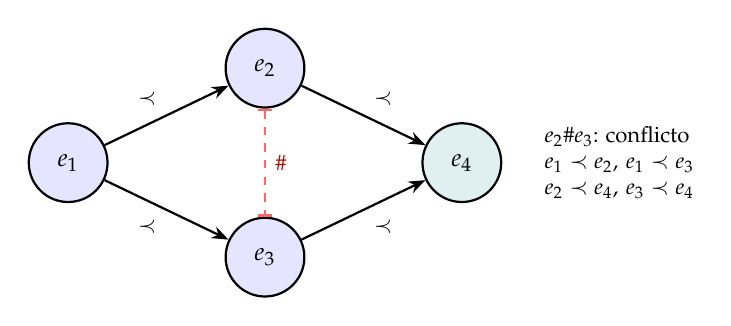
\begin{tikzpicture}[
  ev/.style={circle, draw, thick, minimum size=1cm, font=\small},
  arr/.style={-{Stealth[length=6pt]}, thick},
  conf/.style={draw, dashed, thick, red!60, {Bar[width=5pt]}-{Bar[width=5pt]}}
]
\node[ev, fill=blue!10] (e1) at (0,0) {$e_1$};
\node[ev, fill=blue!10] (e2) at (2.5,1.2) {$e_2$};
\node[ev, fill=blue!10] (e3) at (2.5,-1.2) {$e_3$};
\node[ev, fill=teal!12] (e4) at (5,0) {$e_4$};

\draw[arr] (e1) -- (e2) node[midway, above left, font=\footnotesize] {$\prec$};
\draw[arr] (e1) -- (e3) node[midway, below left, font=\footnotesize] {$\prec$};
\draw[arr] (e2) -- (e4) node[midway, above right, font=\footnotesize] {$\prec$};
\draw[arr] (e3) -- (e4) node[midway, below right, font=\footnotesize] {$\prec$};

\draw[conf] (e2) -- (e3) node[midway, right, font=\footnotesize, red!70!black] {$\#$};

\node[font=\footnotesize, align=left] at (7, 0) {$e_2 \# e_3$: conflicto\\$e_1 \prec e_2,\, e_1 \prec e_3$\\$e_2 \prec e_4,\, e_3 \prec e_4$};
\end{tikzpicture}
\caption{Estructura histórica con cuatro eventos, dos relaciones de precedencia transitivas y un conflicto $e_2 \# e_3$. Los eventos $e_2$ y $e_3$ representan bifurcaciones de la historia que no pueden ocurrir simultáneamente.}
\label{fig:estructura_eventos}
\end{figure}

A partir de esta estructura histórica se pueden definir las entidades del sistema. En Spherepop una entidad no se introduce como un objeto primitivo; se define como una condensación de eventos dentro de la historia~\cite{whitehead,winskel}.

\begin{definition}[Entidad histórica]
\label{def:entidad}
Dado un sistema con estructura histórica $\mathfrak{H}$, una \emph{entidad histórica} es un par $\mathbf{x} = (H(\mathbf{x}), \phi_{\mathbf{x}})$ donde $H(\mathbf{x}) \subseteq E_H$ es el historial de $\mathbf{x}$ y $\phi_{\mathbf{x}}: H(\mathbf{x}) \to \Phi$ es una función que especifica la \emph{contribución estructural} de cada evento al estado de la entidad.
\end{definition}

\begin{definition}[Identidad histórica -- versión refinada]
\label{def:identidad_refinada}
Dos entidades $\mathbf{x}$ e $\mathbf{y}$ son \emph{históricamente idénticas}, escrito $\mathbf{x} =_H \mathbf{y}$, si y sólo si:
\[
H(\mathbf{x}) = H(\mathbf{y}) \quad\text{y}\quad \phi_{\mathbf{x}} = \phi_{\mathbf{y}}.
\]
\end{definition}

La relación parte-todo también puede formularse en términos históricos. Decimos que una entidad $\mathbf{a}$ es parte de una entidad $\mathbf{b}$ si el historial de $\mathbf{a}$ está contenido dentro del historial de $\mathbf{b}$:
\[
\mathbf{a} \preceq_M \mathbf{b} \quad\Longleftrightarrow\quad H(\mathbf{a}) \subseteq H(\mathbf{b}).
\]

Finalmente, la evolución del sistema puede representarse como una expansión progresiva de la historia. Cuando ocurre un nuevo evento $e$, el conjunto de eventos se amplía:
\[
E_{H_{t+1}} = E_{H_t} \cup \{e\}.
\]
La historia crece únicamente a partir de eventos que han ocurrido realmente. No es necesario postular de antemano todas las entidades posibles; las entidades emergen gradualmente conforme la historia se expande~\cite{fowler,kleppmann}.

\section{Restricción histórica y evitación de paradojas}
\label{sec:paradojas}

Una de las motivaciones importantes para adoptar una perspectiva basada en eventos históricos es la dificultad bien conocida que surge cuando los sistemas formales permiten pertenencia global o comprensión irrestricta~\cite{russellparadox,zermelo}. En muchos marcos clásicos se supone la existencia de un universo suficientemente amplio donde cualquier colección definida por una propiedad puede considerarse un objeto legítimo~\cite{frege}. Este tipo de principio resulta extremadamente poderoso pero también conduce a paradojas cuando la definición se aplica de manera reflexiva.

El ejemplo más conocido es la paradoja de Russell~\cite{russellparadox}: si se permite formar libremente conjuntos definidos por cualquier propiedad, se vuelve posible construir la colección de todos los conjuntos que no se contienen a sí mismos, generando una contradicción interna. El problema no surge de un error técnico aislado sino de una suposición estructural: la idea de que todas las colecciones concebibles pueden coexistir dentro de un mismo dominio de pertenencia~\cite{zermelo,vonneumann}.

Spherepop adopta una estrategia distinta. En lugar de permitir que la complejidad del sistema se expanda por definición, restringe su crecimiento a eventos que han ocurrido efectivamente dentro de la historia del sistema. Esta restricción elimina la posibilidad de introducir entidades únicamente por comprensión abstracta. Toda entidad debe estar respaldada por un historial concreto de eventos que haya producido su estructura.

\begin{axiom}[Restricción histórica]
\label{ax:restriccion}
En un sistema Spherepop, toda entidad $\mathbf{x}$ satisface la condición:
\[
H(\mathbf{x}) \subseteq E_H,
\]
donde $E_H$ es el conjunto finito de eventos que han ocurrido efectivamente en la historia del sistema hasta el momento actual. No se permite introducir entidades cuya formación requiera la ocurrencia de eventos que no pertenecen a $E_H$.
\end{axiom}

La clave del Axioma~\ref{ax:restriccion} es que $E_H$ no representa un universo ilimitado de posibilidades, sino únicamente los eventos efectivamente registrados~\cite{fowler}. Cualquier entidad debe corresponder a una configuración histórica derivada de esos eventos.

\begin{theorem}[Ausencia de auto-referencia paradójica]
\label{thm:noparadoja}
En un sistema Spherepop que satisface el Axioma~\ref{ax:restriccion} y donde la relación de precedencia causal $\prec$ es acíclica, no pueden formarse entidades cuya identidad se defina auto-referencialmente mediante su propia historia.
\end{theorem}

\begin{proof}
Supóngase por reducción al absurdo que existe una entidad $\mathbf{x}$ tal que $\mathbf{x} \in H(\mathbf{x})$, es decir, que algún evento en el historial de $\mathbf{x}$ requiere la existencia previa de $\mathbf{x}$ para ocurrir. Por el Axioma~\ref{ax:restriccion}, $H(\mathbf{x}) \subseteq E_H$, y por la Definición~\ref{def:estructura}, $\prec$ es un orden parcial estricto sobre $E_H$, en particular acíclico. La formación de $\mathbf{x}$ requiere que todos sus eventos constitutivos hayan ocurrido con anterioridad causal a la consolidación de $\mathbf{x}$. Si $\mathbf{x}$ fuese requerida por alguno de sus propios eventos constitutivos, existiría un ciclo $e \prec \cdots \prec e$ en $E_H$, contradiciendo la aciclia de $\prec$.
\end{proof}

Desde un punto de vista computacional, este principio se asemeja a sistemas donde la ejecución produce estados acumulativos que dependen de operaciones anteriores~\cite{okasaki,kleppmann}. Un programa no contiene de manera implícita todos los resultados posibles de su ejecución; cada resultado aparece sólo después de que la secuencia correspondiente de operaciones ha ocurrido. La consecuencia filosófica es que el sistema no necesita asumir una ontología infinita desde el inicio~\cite{whitehead}: el dominio de entidades se construye gradualmente a partir de la historia efectiva del sistema.

\section{El axioma de irreversibilidad y espacios de opción}
\label{sec:irreversibilidad}

Gran parte de la teoría contemporánea de la computación describe los sistemas como configuraciones que cambian con el tiempo~\cite{abramsky,plotkin}. Sin embargo, muchos fenómenos cotidianos sugieren que esta descripción es incompleta. Las acciones humanas, las instituciones sociales e incluso los sistemas técnicos dependen profundamente de la historia que los produjo. Dos situaciones pueden parecer idénticas en el presente y, sin embargo, tener consecuencias completamente distintas debido a su pasado~\cite{prigogine,landauer}.

Spherepop formaliza este tipo de situaciones mediante el axioma de irreversibilidad. El principio fundamental establece que los eventos no sólo producen resultados, sino que transforman permanentemente el espacio de posibilidades.

\begin{axiom}[Irreversibilidad]
\label{ax:irreversibilidad}
Sea $\mathcal{X}$ el conjunto de espacios de opción del sistema. Para todo evento irreversible $e: X \to X'$ con $X, X' \in \mathcal{X}$, se tiene:
\[
|X'| \leq |X|,
\]
y en general no existe ningún evento $e^{-1}$ tal que $e^{-1} \circ e = \mathrm{id}_X$. La composición de eventos $H = e_n \circ \cdots \circ e_1 : X_0 \to X_n$ es irreversible como historia completa.
\end{axiom}

\begin{definition}[Espacio de opciones]
\label{def:espacio_opciones}
Un \emph{espacio de opciones} $X$ es un conjunto (finito o infinito) de trayectorias futuras compatibles con todos los eventos que han ocurrido en la historia hasta el momento presente. El espacio inicial $X_0$ representa todas las posibilidades antes de que ocurra ningún evento.
\end{definition}

La figura~\ref{fig:arbol_opciones} representa la dinámica de un espacio de opciones bajo una secuencia de eventos irreversibles.

\begin{figure}[ht]
\centering
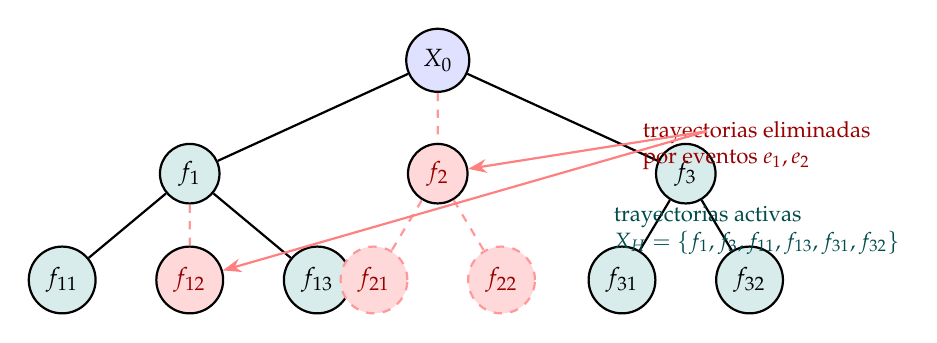
\begin{tikzpicture}[scale=0.9,
  node/.style={circle, draw, thick, minimum size=0.7cm, font=\small},
  level 1/.style={sibling distance=3.5cm, level distance=1.6cm},
  level 2/.style={sibling distance=1.8cm, level distance=1.5cm},
  level 3/.style={sibling distance=1.0cm, level distance=1.4cm},
  eliminated/.style={circle, draw, thick, fill=red!15, minimum size=0.7cm,
                     font=\small, text=red!60!black},
  active/.style={circle, draw, thick, fill=teal!15, minimum size=0.7cm, font=\small},
  arr/.style={thick, -}
]
\node[node, fill=blue!12] (root) {$X_0$}
  child[arr] { node[active] (a1) {$f_1$}
    child[arr] { node[active] (b1) {$f_{11}$} }
    child[arr] { node[eliminated] (b2) {$f_{12}$}
      edge from parent[draw=red!40, dashed]
    }
    child[arr] { node[active] (b3) {$f_{13}$} }
  }
  child[arr] { node[eliminated] (a2) {$f_2$}
    child[arr] { node[eliminated] (b4) {$f_{21}$}
      edge from parent[draw=red!40, dashed]
    }
    child[arr] { node[eliminated] (b5) {$f_{22}$}
      edge from parent[draw=red!40, dashed]
    }
    edge from parent[draw=red!40, dashed]
  }
  child[arr] { node[active] (a3) {$f_3$}
    child[arr] { node[active] (b6) {$f_{31}$} }
    child[arr] { node[active] (b7) {$f_{32}$} }
  };

\node[font=\footnotesize, align=left, right=0.3cm of root] {};
\node[font=\footnotesize, red!60!black, align=left] at (4.5, -1.2)
  {trayectorias eliminadas\\por eventos $e_1, e_2$};
\node[font=\footnotesize, teal!60!black, align=left] at (4.5, -2.4)
  {trayectorias activas\\$X_H = \{f_1, f_3, f_{11}, f_{13}, f_{31}, f_{32}\}$};
\draw[-{Stealth}, thick, red!50] (3.8,-1.0) -- (a2);
\draw[-{Stealth}, thick, red!50] (3.8,-1.0) -- (b2);
\end{tikzpicture}
\caption{Dinámica del espacio de opciones $X_0$ bajo eventos irreversibles. Las trayectorias marcadas en rojo han sido eliminadas por eventos de tipo \emph{pop}. Las trayectorias verdes (activas) constituyen $X_H$, el espacio de opciones compatible con la historia acumulada.}
\label{fig:arbol_opciones}
\end{figure}

Un mundo de Spherepop se describe como una historia compuesta por una secuencia de eventos irreversibles:
\[
H = e_n \circ e_{n-1} \circ \cdots \circ e_1 : X_0 \longrightarrow X_n,
\]
donde $X_0$ representa el espacio inicial de posibilidades y cada $e_i$ es una operación que transforma ese espacio en uno nuevo. El resultado final $X_n$ no es simplemente un estado; es el conjunto de futuros que siguen siendo compatibles con todos los eventos que han ocurrido~\cite{landauer,prigogine}.

En esta formulación, el significado no reside en una configuración instantánea, sino en la trayectoria histórica que conduce a ella~\cite{whitehead,heidegger}. Dos mundos pueden parecer idénticos en un momento dado pero si han sido producidos por historias diferentes no son estructuralmente equivalentes. Su pasado condiciona de manera distinta lo que puede ocurrir después.

\section{Operadores fundamentales de Spherepop}
\label{sec:operadores}

Una vez aceptado el axioma de irreversibilidad, el siguiente paso consiste en describir cómo los eventos modifican el espacio de posibilidades. Spherepop introduce cuatro operadores fundamentales que constituyen la gramática mínima de su cálculo.

\begin{definition}[Operador \emph{pop}]
\label{def:pop}
Sea $X$ un espacio de opciones y $p \in X$ una trayectoria particular. El \emph{operador de exclusión} actúa como:
\[
\mathrm{pop}_p : X \longrightarrow X \setminus \{p\}.
\]
Este operador es irreversible: una vez que $p$ ha sido excluida de $X$, no existe ningún operador del cálculo que restaure $p$ sin introducir un nuevo evento.
\end{definition}

\begin{definition}[Operador \emph{refusal}]
\label{def:refuse}
Sea $R \subseteq X$ un subconjunto de trayectorias que satisfacen una propiedad estructural. El \emph{operador de negativa} actúa como:
\[
\mathrm{refuse}_R : X \longrightarrow X \setminus R = \{x \in X \mid x \notin R\}.
\]
A diferencia de \emph{pop}, que excluye trayectorias individuales, \emph{refusal} excluye clases completas definidas por predicados estructurales~\cite{girard}.
\end{definition}

\begin{definition}[Operador \emph{bind}]
\label{def:bind}
Sean $X$ e $Y$ dos espacios de opciones y $C \subseteq X \times Y$ una relación de compatibilidad. El \emph{operador de ligadura} actúa como:
\[
\mathrm{bind}_C : X \times Y \longrightarrow \{(x,y) \in X \times Y \mid C(x,y)\}.
\]
Este operador introduce dependencias estructurales entre trayectorias de distintos espacios, reduciendo el producto $X \times Y$ al subconjunto compatible~\cite{maclane,girard}.
\end{definition}

\begin{definition}[Operador \emph{collapse}]
\label{def:collapse}
Sea $X$ un espacio de opciones y $\sim$ una relación de equivalencia sobre $X$. El \emph{operador de colapso} actúa como:
\[
\mathrm{collapse}_\sim : X \longrightarrow X/{\sim}.
\]
Este operador comprime la historia identificando trayectorias equivalentes, permitiendo que el sistema represente su historial de manera más compacta sin alterar sus consecuencias causales~\cite{abramsky,turner}.
\end{definition}

La Figura~\ref{fig:operadores} resume la acción de los cuatro operadores sobre un espacio de opciones esquemático.

\begin{figure}[ht]
\centering
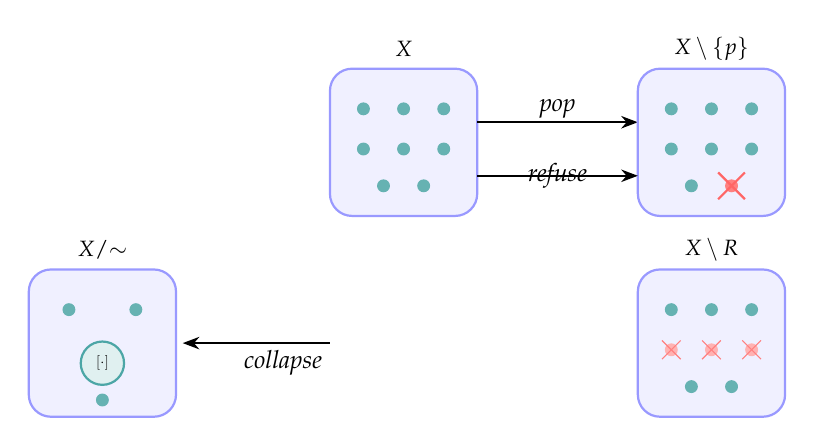
\begin{tikzpicture}[scale=0.85]

\def\drawspace#1#2#3#4{
  \begin{scope}[shift={(#1,#2)}]
    \filldraw[fill=blue!6, draw=blue!40, thick, rounded corners=8pt]
      (-1.1,-1.1) rectangle (1.1,1.1);
    \node[font=\footnotesize\itshape] at (0, 1.4) {#3};
    #4
  \end{scope}
}

\drawspace{0}{0}{$X$}{
  \foreach \x/\y in {-0.6/0.5, 0/0.5, 0.6/0.5, -0.6/-0.1, 0/-0.1, 0.6/-0.1,
                     -0.3/-0.65, 0.3/-0.65}
    \filldraw[teal!60] (\x,\y) circle (2.5pt);
}

\node[font=\small, align=center] at (2.3, 0.5) {\emph{pop}};
\draw[-{Stealth[length=6pt]}, thick] (1.1,0.3) -- (3.5,0.3);

\drawspace{4.6}{0}{$X \setminus \{p\}$}{
  \foreach \x/\y in {-0.6/0.5, 0/0.5, 0.6/0.5, -0.6/-0.1, 0/-0.1, 0.6/-0.1,
                     -0.3/-0.65}
    \filldraw[teal!60] (\x,\y) circle (2.5pt);
  \filldraw[red!50] (0.3,-0.65) circle (2.5pt);
  \draw[red!60, thick] (0.1,-0.85) -- (0.5,-0.45);
  \draw[red!60, thick] (0.5,-0.85) -- (0.1,-0.45);
}

\node[font=\small, align=center] at (2.3, -0.5) {\emph{refuse}};
\draw[-{Stealth[length=6pt]}, thick] (1.1,-0.5) -- (3.5,-0.5);

\drawspace{4.6}{-3}{$X \setminus R$}{
  \foreach \x/\y in {-0.6/0.5, 0/0.5, 0.6/0.5, -0.3/-0.65, 0.3/-0.65}
    \filldraw[teal!60] (\x,\y) circle (2.5pt);
  \foreach \x/\y in {-0.6/-0.1, 0/-0.1, 0.6/-0.1}
    { \filldraw[red!30] (\x,\y) circle (2.5pt);
      \draw[red!50, thin] (\x-0.14,\y-0.14) -- (\x+0.14,\y+0.14);
      \draw[red!50, thin] (\x+0.14,\y-0.14) -- (\x-0.14,\y+0.14); }
}

\node[font=\small, align=center] at (-1.8, -3.3) {\emph{collapse}};
\draw[-{Stealth[length=6pt]}, thick] (-1.1,-3.0) -- (-3.3,-3.0);

\drawspace{-4.5}{-3}{$X/{\sim}$}{
  \filldraw[teal!60] (-0.5,0.5) circle (2.5pt);
  \filldraw[teal!60] (0.5,0.5) circle (2.5pt);
  \node[circle, draw=teal!70, thick, minimum size=0.55cm, fill=teal!12]
    at (0,-0.3) {};
  \node[font=\tiny] at (0,-0.3) {$[\cdot]$};
  \filldraw[teal!60] (0,-0.85) circle (2.5pt);
}

\end{tikzpicture}
\caption{Acción esquemática de los cuatro operadores fundamentales de Spherepop sobre un espacio de opciones. \emph{Pop} elimina una trayectoria individual (marcada en rojo). \emph{Refuse} elimina un subconjunto $R$ definido estructuralmente. \emph{Collapse} identifica trayectorias equivalentes bajo $\sim$ (representadas por la clase de equivalencia $[\cdot]$). El operador \emph{bind} actúa sobre productos de espacios y no se muestra en esta figura bidimensional.}
\label{fig:operadores}
\end{figure}

\begin{proposition}[Monotonía decreciente de la opcionalidad]
\label{prop:monotonia}
Los cuatro operadores fundamentales son monotónicamente decrecientes con respecto al tamaño del espacio de opciones:
\[
|\mathrm{pop}_p(X)| \leq |X|, \quad
|\mathrm{refuse}_R(X)| \leq |X|, \quad
|\mathrm{collapse}_\sim(X)| \leq |X|.
\]
Para \emph{bind}: $|\mathrm{bind}_C(X \times Y)| \leq |X \times Y| = |X| \cdot |Y|$.
\end{proposition}

\begin{proof}
Cada operador produce un subconjunto o cociente del espacio original. $\mathrm{pop}_p(X) = X \setminus \{p\}$ tiene a lo sumo $|X| - 1$ elementos si $p \in X$ y $|X|$ si $p \notin X$. $\mathrm{refuse}_R(X) = X \setminus R$ tiene a lo sumo $|X|$ elementos. $\mathrm{collapse}_\sim(X) = X/{\sim}$ tiene a lo sumo $|X|$ clases de equivalencia, con igualdad si y sólo si $\sim$ es la identidad. $\mathrm{bind}_C(X \times Y) \subseteq X \times Y$ de manera inmediata.
\end{proof}

\section{Construcción de compuertas lógicas}
\label{sec:logica}

Una vez definidos los operadores fundamentales de Spherepop, resulta posible mostrar que estructuras lógicas elementales pueden surgir directamente de la dinámica de restricción de espacios de opción. Esta observación es importante porque sugiere que la lógica no necesita introducirse como un sistema axiomático independiente; puede aparecer como una consecuencia estructural de eventos irreversibles que restringen futuros posibles~\cite{girard,abramsky}.

Si $X$ es un espacio de opciones y $A \subseteq X$ es la región correspondiente a la proposición $A$ (es decir, el conjunto de trayectorias futuras en las que $A$ es verdadera), entonces las operaciones lógicas se interpretan geométricamente como sigue.

\begin{definition}[Interpretación lógica de los operadores]
\label{def:logica}
Sea $X$ un espacio de opciones y $A, B \subseteq X$ regiones proposicionales. Se definen:
\[
\neg A = X \setminus A, \qquad A \land B = A \cap B, \qquad A \lor B = A \cup B, \qquad A \Rightarrow B = (X \setminus A) \cup B.
\]
\end{definition}

\begin{figure}[ht]
\centering
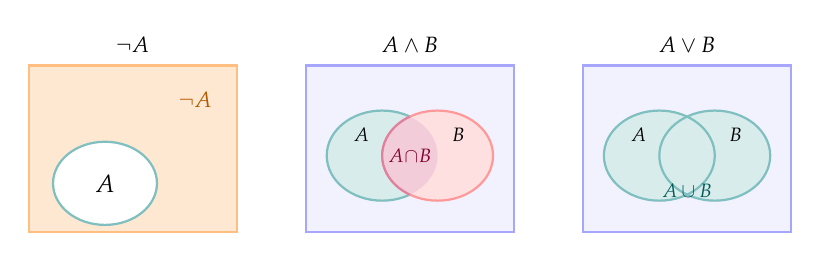
\begin{tikzpicture}[scale=0.88]

\begin{scope}[shift={(0,0)}]
  \filldraw[fill=blue!5, draw=blue!35, thick] (-1.5,-1.2) rectangle (1.5,1.2);
  \node[font=\footnotesize\itshape] at (0,1.5) {$\neg A$};
  \filldraw[fill=teal!18, draw=teal!50, thick] (-0.4,-0.5) ellipse (0.75cm and 0.6cm);
  \node[font=\small] at (-0.4,-0.5) {$A$};
  \filldraw[fill=gray!15, draw=gray!50, thick, opacity=0.5]
    (-1.5,-1.2) rectangle (1.5,1.2);
  \filldraw[fill=white, draw=none]
    (-0.4,-0.5) ellipse (0.75cm and 0.6cm);
  \filldraw[fill=orange!18, draw=orange!50, thick]
    (-1.5,-1.2) rectangle (1.5,1.2);
  \filldraw[fill=white, draw=teal!50, thick]
    (-0.4,-0.5) ellipse (0.75cm and 0.6cm);
  \node[font=\small] at (-0.4,-0.5) {$A$};
  \node[font=\footnotesize, orange!70!black] at (0.9,0.7) {$\neg A$};
\end{scope}

\begin{scope}[shift={(4,0)}]
  \filldraw[fill=blue!5, draw=blue!35, thick] (-1.5,-1.2) rectangle (1.5,1.2);
  \node[font=\footnotesize\itshape] at (0,1.5) {$A \land B$};
  \filldraw[fill=teal!15, draw=teal!50, thick] (-0.4,-0.1) ellipse (0.8cm and 0.65cm);
  \filldraw[fill=red!12, draw=red!40, thick] (0.4,-0.1) ellipse (0.8cm and 0.65cm);
  \begin{scope}
    \clip (-0.4,-0.1) ellipse (0.8cm and 0.65cm);
    \filldraw[fill=purple!20, draw=purple!50, thick]
      (0.4,-0.1) ellipse (0.8cm and 0.65cm);
  \end{scope}
  \node[font=\scriptsize] at (-0.7,0.2) {$A$};
  \node[font=\scriptsize] at (0.7,0.2) {$B$};
  \node[font=\scriptsize, purple!70!black] at (0,-0.1) {$A\!\cap\! B$};
\end{scope}

\begin{scope}[shift={(8,0)}]
  \filldraw[fill=blue!5, draw=blue!35, thick] (-1.5,-1.2) rectangle (1.5,1.2);
  \node[font=\footnotesize\itshape] at (0,1.5) {$A \lor B$};
  \begin{scope}
    \clip (-1.5,-1.2) rectangle (1.5,1.2);
    \filldraw[fill=teal!15, draw=none] (-0.4,-0.1) ellipse (0.8cm and 0.65cm);
    \filldraw[fill=teal!15, draw=none] (0.4,-0.1) ellipse (0.8cm and 0.65cm);
  \end{scope}
  \draw[teal!50, thick] (-0.4,-0.1) ellipse (0.8cm and 0.65cm);
  \draw[teal!50, thick] (0.4,-0.1) ellipse (0.8cm and 0.65cm);
  \node[font=\scriptsize] at (-0.7,0.2) {$A$};
  \node[font=\scriptsize] at (0.7,0.2) {$B$};
  \node[font=\scriptsize, teal!70!black] at (0,-0.6) {$A \cup B$};
\end{scope}

\end{tikzpicture}
\caption{Interpretación geométrica de las operaciones lógicas sobre espacios de opciones. La negación $\neg A$ corresponde al complemento de $A$ en $X$ (región naranja). La conjunción $A \land B$ corresponde a la intersección (región púrpura). La disyunción $A \lor B$ corresponde a la unión de ambas regiones.}
\label{fig:logica_geometrica}
\end{figure}

\begin{theorem}[Completitud lógica]
\label{thm:completitud_logica}
Las operaciones de la Definición~\ref{def:logica} satisfacen las leyes de la lógica proposicional clásica. En particular, $(\mathcal{P}(X), \cap, \cup, \complement_X, \emptyset, X)$ es una álgebra de Boole, donde $\mathcal{P}(X)$ denota el conjunto potencia de $X$~\cite{birkhoff}.
\end{theorem}

\begin{proof}
Es resultado estándar que el conjunto potencia de cualquier conjunto forma un álgebra de Boole con la intersección, la unión y el complemento relativo~\cite{birkhoff,maclane}. La interpretación de la Definición~\ref{def:logica} mapea las operaciones lógicas exactamente a estas operaciones, de donde se sigue la completitud.
\end{proof}

La observación central es que la lógica emerge aquí como una propiedad estructural de los espacios de opción~\cite{girard}, no como un sistema axiomático independiente. Las compuertas lógicas no son más que configuraciones particulares de restricciones históricas. En contextos cotidianos, estas operaciones aparecen constantemente: cuando alguien afirma ``si llueve llevaré paraguas'' está introduciendo una dependencia estructural $A \Rightarrow B$; cuando descarta una opción durante una deliberación aplica una exclusión $\mathrm{pop}$; cuando mantiene varias alternativas abiertas preserva una disyunción de futuros.

\section{Un lenguaje mínimo basado en pila}
\label{sec:pila}

Una vez que las operaciones fundamentales de Spherepop se han interpretado como transformaciones lógicas sobre espacios de opción, el siguiente paso consiste en organizarlas dentro de una estructura computacional explícita. Una forma particularmente natural de hacerlo es mediante una máquina basada en pila, similar en espíritu a los lenguajes concatenativos como Forth~\cite{moore,okasaki,turner}.

Los lenguajes basados en pila poseen una propiedad conceptual importante para Spherepop. En ellos, los programas no se describen como funciones que reciben argumentos nombrados, sino como secuencias de operaciones que transforman una estructura acumulativa~\cite{moore}. Cada operación toma elementos de la pila, los transforma y deposita el resultado nuevamente en ella. El estado del sistema no se describe mediante variables globales sino mediante el historial de transformaciones aplicadas, lo cual coincide de manera precisa con la lógica histórica de Spherepop.

\begin{definition}[Máquina de pila de Spherepop]
\label{def:maquina_pila}
Una \emph{máquina de pila de Spherepop} (MPS) es una estructura $\mathcal{M} = (Q, \Sigma, \Gamma, \delta, q_0, S_0)$ donde:
\begin{itemize}
\item[] $Q$ es el conjunto finito de estados de control,
\item[] $\Sigma = \{\mathrm{pop}, \mathrm{refuse}, \mathrm{bind}, \mathrm{collapse}\}$ es el alfabeto de operadores,
\item[] $\Gamma$ es el conjunto de espacios de opción que pueden aparecer en la pila,
\item[] $\delta: Q \times \Sigma \times \Gamma^* \to Q \times \Gamma^*$ es la función de transición,
\item[] $q_0 \in Q$ es el estado inicial, y
\item[] $S_0 = (X_0)$ es la configuración inicial de la pila con un único espacio de opciones $X_0$.
\end{itemize}
\end{definition}

\begin{definition}[Configuración y cómputo]
\label{def:computo}
Una \emph{configuración} de la MPS es un par $(q, S)$ donde $q \in Q$ y $S = (X_1, \ldots, X_n) \in \Gamma^*$ es la pila actual. Un \emph{cómputo} es una secuencia de configuraciones
\[
(q_0, S_0) \vdash (q_1, S_1) \vdash \cdots \vdash (q_k, S_k)
\]
donde cada transición $(q_i, S_i) \vdash (q_{i+1}, S_{i+1})$ corresponde a la aplicación de algún operador $o_i \in \Sigma$.
\end{definition}

La Figura~\ref{fig:pila_ejecucion} ilustra la ejecución de una secuencia de operadores sobre la pila.

\begin{figure}[ht]
\centering
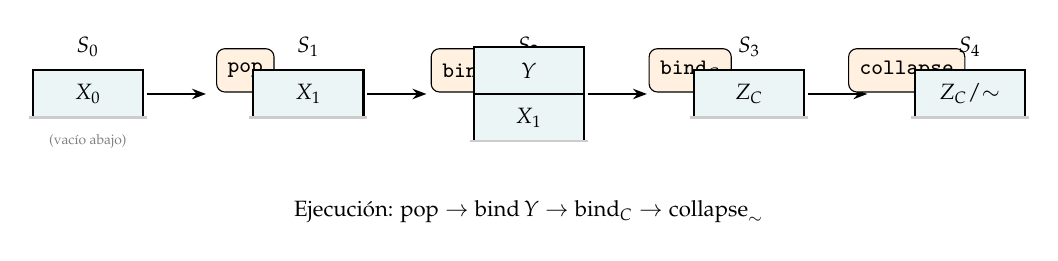
\begin{tikzpicture}[
  stack/.style={rectangle, draw, thick, minimum width=1.4cm, minimum height=0.6cm,
               font=\footnotesize, fill=teal!8},
  op/.style={rectangle, draw, rounded corners=3pt, fill=orange!12,
             font=\footnotesize\ttfamily, minimum height=0.55cm, inner sep=4pt},
  arr/.style={-{Stealth[length=5pt]}, thick}
]

\begin{scope}[shift={(0,0)}]
  \node[font=\footnotesize\itshape] at (0, 1.8) {$S_0$};
  \node[stack] at (0,1.2) {$X_0$};
  \node[font=\tiny, gray] at (0,0.6) {(vacío abajo)};
  \draw[thick, gray!40] (-0.75,0.9) -- (0.75,0.9);
\end{scope}

\draw[arr] (0.75,1.2) -- (1.5,1.2);
\node[op] at (2.0,1.5) {pop};

\begin{scope}[shift={(2.8,0)}]
  \node[font=\footnotesize\itshape] at (0,1.8) {$S_1$};
  \node[stack] at (0,1.2) {$X_1$};
  \draw[thick, gray!40] (-0.75,0.9) -- (0.75,0.9);
\end{scope}

\draw[arr] (3.55,1.2) -- (4.3,1.2);
\node[op] at (4.8,1.5) {bind};

\begin{scope}[shift={(5.6,0)}]
  \node[font=\footnotesize\itshape] at (0,1.8) {$S_2$};
  \node[stack] at (0,1.5) {$Y$};
  \node[stack] at (0,0.9) {$X_1$};
  \draw[thick, gray!40] (-0.75,0.6) -- (0.75,0.6);
\end{scope}

\draw[arr] (6.35,1.2) -- (7.1,1.2);
\node[op] at (7.65,1.5) {bind$_C$};

\begin{scope}[shift={(8.4,0)}]
  \node[font=\footnotesize\itshape] at (0,1.8) {$S_3$};
  \node[stack] at (0,1.2) {$Z_C$};
  \draw[thick, gray!40] (-0.75,0.9) -- (0.75,0.9);
\end{scope}

\draw[arr] (9.15,1.2) -- (9.9,1.2);
\node[op] at (10.4,1.5) {collapse};

\begin{scope}[shift={(11.2,0)}]
  \node[font=\footnotesize\itshape] at (0,1.8) {$S_4$};
  \node[stack] at (0,1.2) {$Z_C/{\sim}$};
  \draw[thick, gray!40] (-0.75,0.9) -- (0.75,0.9);
\end{scope}

\node[font=\footnotesize, align=center] at (5.6, -0.3)
  {Ejecución: $\mathrm{pop} \to \mathrm{bind}\,Y \to \mathrm{bind}_C \to \mathrm{collapse}_\sim$};
\end{tikzpicture}
\caption{Ejecución de una secuencia de operadores sobre la pila de una MPS. El estado inicial contiene el espacio $X_0$. Tras \emph{pop} se obtiene $X_1 \subsetneq X_0$. \emph{bind} introduce un segundo espacio $Y$ en la pila. $\mathrm{bind}_C$ combina ambos en $Z_C = \mathrm{bind}_C(X_1, Y)$. \emph{collapse} produce la pila final con el cociente $Z_C / {\sim}$.}
\label{fig:pila_ejecucion}
\end{figure}

\begin{definition}[Programa Spherepop]
\label{def:programa}
Un \emph{programa Spherepop} es una secuencia finita de operadores
\[
P = (o_1, o_2, \ldots, o_k), \quad o_i \in \Sigma^* \cup \{\text{definiciones}\}.
\]
La \emph{semántica denotacional} de $P$ es la función
\[
\llbracket P \rrbracket = o_k \circ \cdots \circ o_1 : \Gamma^* \to \Gamma^*
\]
sobre el espacio de configuraciones de pila~\cite{plotkin,abramsky}.
\end{definition}

\section{Una máquina mínima de cálculo}
\label{sec:maquina}

A partir de la estructura basada en pila introducida en la sección anterior es posible definir una máquina de cálculo mínima cuya dinámica está gobernada únicamente por operadores de Spherepop. Esta máquina no se define en términos de registros, direcciones de memoria o instrucciones imperativas tradicionales; en cambio, se define mediante transformaciones sucesivas del espacio de opciones que representa el contexto computacional~\cite{moore,turner}.

El estado de la máquina en un momento dado consiste en una pila finita
\[
S = (X_1, X_2, \ldots, X_n)
\]
donde cada elemento $X_i$ representa un espacio de opciones compatible con la historia acumulada hasta ese punto del cálculo. Un programa puede representarse como una secuencia finita de operadores
\[
P = (o_1, o_2, \ldots, o_k)
\]
y la ejecución del programa produce una secuencia de estados de pila:
\[
S_{i+1} = o_i(S_i), \quad i = 0, 1, \ldots, k-1.
\]

\begin{theorem}[Completitud computacional de la MPS]
\label{thm:completitud}
La máquina de pila de Spherepop con los cuatro operadores fundamentales es computacionalmente completa en el sentido de que puede simular cualquier máquina de Turing~\cite{turing}, dado que los lenguajes concatenativos basados en pila con capacidad de definición de palabras y bifurcación condicional son Turing-completos~\cite{moore,turner}.
\end{theorem}

\begin{proof}[Esbozo de demostración]
La demostración sigue la estrategia estándar para lenguajes concatenativos~\cite{moore}: se muestra que la MPS puede simular las instrucciones de una máquina de Turing universal. Específicamente: (1) el operador \emph{bind} puede usarse para representar la cinta de la máquina de Turing como una estructura de pares dependientes; (2) \emph{pop} y \emph{refuse} implementan la función de transición eliminando configuraciones no-objetivo del espacio de opciones; (3) \emph{collapse} permite la representación compacta de estados de cómputo equivalentes; (4) la composición secuencial de operadores permite implementar bucles mediante definición recursiva de palabras, en analogía con el mecanismo de \texttt{:} en Forth~\cite{moore}. La completitud se hereda del resultado de Turing-completitud de los lenguajes concatenativos con recursión primitiva~\cite{turner}.
\end{proof}

\section{Nombres, funciones y trayectorias históricas}
\label{sec:nombres}

La construcción de una máquina de cálculo basada en la historia permite reinterpretar conceptos fundamentales de la programación desde una perspectiva distinta~\cite{church,plotkin,okasaki}. En particular, nociones tan familiares como función, variable y nombre pueden entenderse como mecanismos para estabilizar trayectorias dentro del espacio de opciones.

Asignar un nombre a una función puede interpretarse como un acto de fijación histórica. El nombre identifica una trayectoria específica dentro del espacio de transformaciones posibles~\cite{church}. Formalmente, un nombre puede representarse como una referencia a una historia específica de transformaciones:
\[
f = e_k \circ \cdots \circ e_2 \circ e_1 : X \longrightarrow X'.
\]
Cuando el nombre $f$ aparece en un programa, el sistema aplica nuevamente esta composición de eventos sobre el espacio de opciones actual.

\begin{definition}[Vocabulario de Spherepop]
\label{def:vocabulario}
El \emph{vocabulario} del sistema en un momento dado es un conjunto parcialmente ordenado
\[
\mathcal{V} = \{(f_i, H_{f_i})\}_{i \in I}
\]
donde cada $f_i$ es un nombre y $H_{f_i}$ es la historia de transformaciones que ese nombre denota. El vocabulario crece de manera acumulativa: nuevas palabras se añaden pero las ya definidas mantienen su historial fijo.
\end{definition}

\begin{remark}
En lenguajes concatenativos como Forth, las palabras del vocabulario corresponden precisamente a secuencias nombradas de operaciones sobre la pila~\cite{moore}. El vocabulario del lenguaje es, en esencia, un conjunto de trayectorias históricas que pueden ser reutilizadas y combinadas. Spherepop adopta una interpretación aún más literal de esta idea: las palabras del sistema no representan simplemente procedimientos abstractos sino historias de transformación del espacio de opciones. Invocar una palabra equivale a reenactuar esa historia dentro del contexto actual del sistema, en un sentido análogo al que Austin denomina los actos de habla ilocucionarios~\cite{austin}.
\end{remark}

La Figura~\ref{fig:vocabulario} ilustra la estructura del vocabulario como una red de historias reutilizables.

\begin{figure}[ht]
\centering
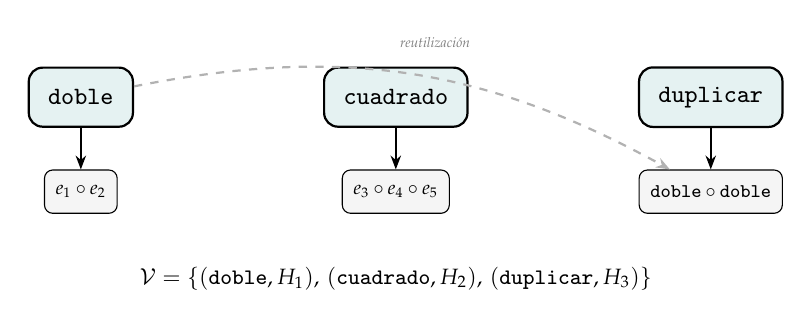
\begin{tikzpicture}[
  word/.style={rectangle, draw, thick, rounded corners=5pt, fill=teal!10,
               minimum height=0.75cm, font=\small\ttfamily, inner sep=7pt},
  hist/.style={rectangle, draw, rounded corners=3pt, fill=gray!8,
               font=\scriptsize, inner sep=4pt, minimum height=0.55cm},
  arr/.style={-{Stealth[length=5pt]}, thick},
  compose/.style={-{Stealth[length=5pt]}, thick, dashed, gray!60}
]

\node[word] (w1) at (0,0) {doble};
\node[word] (w2) at (4,0) {cuadrado};
\node[word] (w3) at (8,0) {duplicar};

\node[hist] (h1) at (0,-1.2) {$e_1 \circ e_2$};
\node[hist] (h2) at (4,-1.2) {$e_3 \circ e_4 \circ e_5$};
\node[hist] (h3) at (8,-1.2) {$\mathtt{doble} \circ \mathtt{doble}$};

\draw[arr] (w1) -- (h1);
\draw[arr] (w2) -- (h2);
\draw[arr] (w3) -- (h3);

\draw[compose] (w1) to[bend left=20] (h3);
\node[font=\tiny\itshape, gray] at (4.5,0.7) {reutilización};

\node[font=\footnotesize, align=center] at (4,-2.3)
  {$\mathcal{V} = \{(\mathtt{doble}, H_1),\,(\mathtt{cuadrado}, H_2),\,(\mathtt{duplicar}, H_3)\}$};
\end{tikzpicture}
\caption{Vocabulario de Spherepop como red de historias reutilizables. Cada palabra nombrada ($\mathtt{doble}$, $\mathtt{cuadrado}$, $\mathtt{duplicar}$) está vinculada a una historia de transformaciones. La palabra $\mathtt{duplicar}$ reutiliza la historia de $\mathtt{doble}$ como componente.}
\label{fig:vocabulario}
\end{figure}

\section{Métrica de opcionalidad y entropía histórica}
\label{sec:opcionalidad}

El cálculo de Spherepop introduce una perspectiva en la cual la evolución de un sistema puede interpretarse como una reducción progresiva del espacio de futuros posibles. Esta observación sugiere la posibilidad de definir una magnitud cuantitativa que mida la cantidad de opcionalidad disponible en un momento determinado de la historia~\cite{landauer,bennett,shannon}.

\begin{definition}[Métrica de opcionalidad]
\label{def:opcionalidad}
Sea $H$ una historia de eventos y $X_H$ el espacio de opciones compatible con esa historia. La \emph{opcionalidad} del sistema en el estado $H$ se define como:
\[
\mathcal{O}(H) = \log |X_H|
\]
donde $|X_H|$ representa el número de trayectorias futuras compatibles con la historia $H$. En el caso en que $X_H$ posee una medida de probabilidad $\mu$ sobre sus trayectorias, la opcionalidad se refina como:
\[
\mathcal{O}_\mu(H) = -\sum_{x \in X_H} p(x) \log p(x),
\]
donde $p = d\mu$ es la función de masa de probabilidad discreta.
\end{definition}

\begin{remark}
La Definición~\ref{def:opcionalidad} es análoga a la entropía de Shannon~\cite{shannon}: mide la incertidumbre estructural del sistema respecto a su futuro. En el contexto de Spherepop, la opcionalidad mide la cantidad de futuros disponibles antes de que nuevas decisiones o eventos restrinjan el sistema.
\end{remark}

\begin{proposition}[Decrecimiento de la opcionalidad]
\label{prop:decrecimiento}
Sea $H' = H \cup \{e\}$ la historia extendida por un evento irreversible $e$. Entonces:
\[
\mathcal{O}(H') \leq \mathcal{O}(H).
\]
La desigualdad es estricta si y sólo si $e$ elimina al menos una trayectoria de $X_H$.
\end{proposition}

\begin{proof}
Por el Axioma~\ref{ax:irreversibilidad}, $|X_{H'}| \leq |X_H|$, de donde $\log|X_{H'}| \leq \log|X_H|$. La desigualdad es estricta si y sólo si $|X_{H'}| < |X_H|$, es decir, si $e$ elimina al menos una trayectoria de $X_H$ al producir $X_{H'} \subsetneq X_H$.
\end{proof}

La Figura~\ref{fig:opcionalidad} ilustra la evolución de la opcionalidad a lo largo de una historia de eventos.

\begin{figure}[ht]
\centering
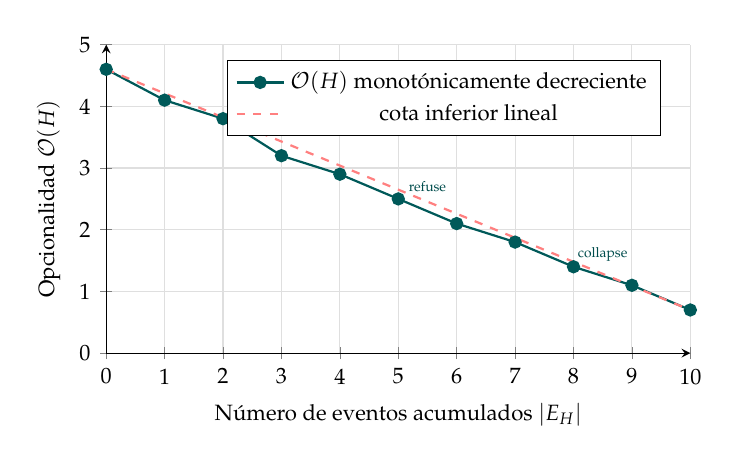
\begin{tikzpicture}
\begin{axis}[
  width=9cm, height=5.5cm,
  xlabel={Número de eventos acumulados $|E_H|$},
  ylabel={Opcionalidad $\mathcal{O}(H)$},
  xmin=0, xmax=10,
  ymin=0, ymax=5,
  xtick={0,1,2,3,4,5,6,7,8,9,10},
  ytick={0,1,2,3,4,5},
  grid=major,
  grid style={gray!25},
  axis lines=left,
  tick label style={font=\footnotesize},
  label style={font=\footnotesize},
  legend style={font=\footnotesize, at={(0.95,0.95)}, anchor=north east}
]
\addplot[thick, teal!70!black, mark=*, mark size=2pt]
  coordinates {(0,4.6) (1,4.1) (2,3.8) (3,3.2) (4,2.9) (5,2.5) (6,2.1) (7,1.8) (8,1.4) (9,1.1) (10,0.7)};
\addlegendentry{$\mathcal{O}(H)$ monotónicamente decreciente}

\addplot[thick, red!50, dashed, domain=0:10, samples=50]
  {4.6 - 0.39*x};
\addlegendentry{cota inferior lineal}

\node[font=\tiny, teal!60!black] at (axis cs:2.5,4.0) {$\mathrm{pop}$};
\node[font=\tiny, teal!60!black] at (axis cs:5.5,2.7) {$\mathrm{refuse}$};
\node[font=\tiny, teal!60!black] at (axis cs:8.5,1.6) {$\mathrm{collapse}$};
\end{axis}
\end{tikzpicture}
\caption{Evolución monótonamente decreciente de la opcionalidad $\mathcal{O}(H)$ a lo largo de una historia de eventos. Cada evento reduce (o mantiene) la opcionalidad disponible. Los eventos de tipo \emph{pop} y \emph{refuse} producen decrementos más abruptos; \emph{collapse} puede producir decrementos más suaves al identificar trayectorias equivalentes.}
\label{fig:opcionalidad}
\end{figure}

\begin{remark}[Conexión con el principio de Landauer]
La Proposición~\ref{prop:decrecimiento} conecta con el principio de Landauer~\cite{landauer}, según el cual la eliminación irreversible de información implica una disipación mínima de energía proporcional a $k_B T \ln 2$ por bit eliminado, donde $k_B$ es la constante de Boltzmann y $T$ es la temperatura. En el contexto de Spherepop, los eventos de tipo \emph{pop} corresponden exactamente a operaciones de borrado irreversible en el sentido de Landauer: eliminan una trayectoria del espacio de opciones y esa eliminación no puede revertirse sin la ocurrencia de un nuevo evento constitutivo. Bennett~\cite{bennett} demostró que el cómputo reversible puede evitar este costo, lo cual en el lenguaje de Spherepop significa que existen secuencias de eventos que conservan la opcionalidad ($\mathcal{O}(H') = \mathcal{O}(H)$). Sin embargo, el Axioma~\ref{ax:irreversibilidad} establece que las historias de Spherepop son en general irreversibles, de manera que la reducción de opcionalidad es la regla y su conservación es el caso especial.
\end{remark}

\section{Implicaciones para sistemas cognitivos, computacionales y sociales}
\label{sec:implicaciones}

El enfoque histórico de Spherepop no se limita a una reformulación abstracta de la estructura matemática. También ofrece un marco conceptual particularmente adecuado para describir sistemas reales donde la historia irreversible desempeña un papel central. En muchos dominios, desde la cognición hasta la organización social y los sistemas computacionales distribuidos, los estados observables sólo adquieren sentido cuando se interpretan a la luz de la trayectoria que los produjo~\cite{prigogine,heidegger,kleppmann}.

En los sistemas cognitivos, la percepción y el significado no aparecen como entidades estáticas. La comprensión de una situación depende de la secuencia de experiencias previas que han configurado el contexto interpretativo del agente~\cite{searle,fodor}. Un recuerdo, una asociación o una expectativa no es simplemente un dato almacenado en una estructura fija; es la sedimentación de múltiples eventos de aprendizaje, atención y acción. Dos individuos pueden percibir el mismo estímulo sensorial y, sin embargo, interpretarlo de manera distinta porque sus historias cognitivas difieren~\cite{goffman}. Desde la perspectiva de Spherepop, estas diferencias no son anomalías del sistema sino consecuencias naturales de trayectorias históricas distintas, formalizables mediante la Definición~\ref{def:identidad} de identidad histórica.

En los sistemas computacionales contemporáneos, la dependencia de la historia resulta igualmente evidente~\cite{lamport,kleppmann}. Los sistemas de control de versiones, las arquitecturas basadas en \emph{event sourcing}~\cite{fowler} y las cadenas de bloques~\cite{nakamoto} funcionan precisamente porque cada estado del sistema se deriva de una secuencia verificable de operaciones anteriores. La consistencia no se define únicamente por la configuración actual del sistema, sino por la posibilidad de reconstruir la historia que condujo a esa configuración. Los tipos de datos replicados libres de conflicto~\cite{shapiro} extienden esta idea al caso distribuido, donde múltiples historiales parciales deben reconciliarse de manera consistente. Spherepop proporciona una manera natural de formalizar este tipo de estructuras, ya que coloca la historia en el centro de la definición del sistema.

En el ámbito social, la dependencia de la historia resulta aún más evidente~\cite{searle,austin,goffman}. Instituciones, normas y relaciones no existen como estructuras abstractas independientes del tiempo; se forman mediante acuerdos, conflictos, decisiones y transformaciones que dejan rastros históricos~\cite{searle}. Un tratado político, una ley o una tradición cultural adquieren significado porque pueden vincularse con una secuencia reconocible de acontecimientos. Incluso cuando las instituciones parecen estables, su identidad depende de la continuidad de su historia, en el sentido de la Definición~\ref{def:identidad_refinada}.

Spherepop permite describir estos fenómenos de manera unificada porque trata la identidad, la estructura y la composición como consecuencias de trayectorias históricas. Formalmente, cualquier sistema modelado dentro de Spherepop puede describirse como una historia $H = (E_H, \prec)$ a partir de la cual emergen las entidades, las relaciones y los ámbitos. Las entidades se identifican con subconjuntos históricos $H(\mathbf{x})$, las relaciones parte-todo se derivan de inclusiones entre estos subconjuntos (Definición~\ref{def:mereologia}) y las estructuras de alcance se representan mediante ámbitos anidados que delimitan regiones de la historia (Definición~\ref{def:burbuja}).

Al adoptar esta perspectiva, Spherepop propone una base conceptual donde significado, identidad y computación se comprenden como manifestaciones de una misma lógica histórica: lo que algo es depende de lo que le ha ocurrido; lo que un sistema puede hacer depende de los eventos que han configurado su estructura; y la complejidad que observamos en el mundo no surge de axiomas atemporales sino de la acumulación irreversible de acciones.

\section{Interpretación categórica}
\label{sec:categorica}

La estructura histórica de Spherepop admite una interpretación natural dentro del marco de la teoría de categorías~\cite{maclane,awodey,jacobs}. Esta interpretación permite formalizar la composición de historias y la transformación de espacios de opción mediante morfismos, conectando el cálculo con semánticas más abstractas de sistemas computacionales.

\begin{definition}[Categoría de historias de Spherepop]
\label{def:categoria}
La \emph{categoría de historias de Spherepop}, denotada $\mathbf{Sph}$, se define como sigue:
\begin{itemize}
\item[] Los \emph{objetos} son espacios de opciones $X, Y, Z \in \mathcal{X}$.
\item[] Los \emph{morfismos} $f: X \to Y$ son eventos irreversibles (o composiciones finitas de ellos) que transforman el espacio $X$ en el espacio $Y$.
\item[] La \emph{composición} $g \circ f: X \to Z$ de morfismos $f: X \to Y$ y $g: Y \to Z$ corresponde a la secuencia histórica de ambos eventos.
\item[] El \emph{morfismo identidad} $\mathrm{id}_X: X \to X$ representa la historia trivial donde no ocurre ningún evento.
\end{itemize}
\end{definition}

\begin{proposition}
\label{prop:categoria}
$\mathbf{Sph}$ es una categoría en el sentido de Mac Lane~\cite{maclane}. La asociatividad de la composición se sigue de la asociatividad de la secuenciación histórica, y las identidades satisfacen las leyes unitarias por definición.
\end{proposition}

La Figura~\ref{fig:diagrama_categoria} presenta el diagrama conmutativo básico de la categoría $\mathbf{Sph}$.

\begin{figure}[ht]
\centering
\begin{tikzcd}[row sep=2.5cm, column sep=3cm, font=\small]
X \arrow[r, "f"] \arrow[dr, "g \circ f"'] & Y \arrow[d, "g"] \\
& Z
\end{tikzcd}
\caption{Diagrama conmutativo en $\mathbf{Sph}$. La composición de morfismos corresponde a la concatenación de historias: $g \circ f: X \to Z$ es la historia que primero aplica $f$ y luego $g$.}
\label{fig:diagrama_categoria}
\end{figure}

\begin{definition}[Funtor de realización]
\label{def:funtor}
Sea $\mathbf{Set}$ la categoría de conjuntos. El \emph{funtor de realización}
\[
\mathcal{R}: \mathbf{Sph} \longrightarrow \mathbf{Set}
\]
envía cada espacio de opciones $X \in \mathbf{Sph}$ al conjunto subyacente de trayectorias $|X|$, y cada morfismo $f: X \to Y$ a la función de restricción $|f|: |X| \to |Y|$ inducida por el operador $f$.
\end{definition}

\begin{remark}
La interpretación categórica de Spherepop permite conectar el cálculo con marcos más generales utilizados en semántica computacional, como las categorías de dominios de Scott~\cite{scottdana,abramsky} y las categorías de juegos de Abramsky~\cite{abramsky}. En particular, la irreversibilidad de los morfismos en $\mathbf{Sph}$ distingue esta categoría de las categorías de procesos reversibles estudiadas en cómputo cuántico~\cite{baez}, estableciendo un contraste productivo con ese programa.
\end{remark}

\section{Conclusión}
\label{sec:conclusion}

Este ensayo ha presentado Spherepop como un marco conceptual, visual y formal que comienza con eventos irreversibles en lugar de estados o conjuntos atemporales. La inversión del punto de partida, respecto de las tradiciones formales basadas en pertenencia abstracta~\cite{cantor,zermelo} o en sistemas de tipos atemporales~\cite{martinlof,homotopy}, no es un accidente estilístico sino una apuesta filosófica y técnica central.

A partir de esta inversión se ha mostrado cómo la estructura puede entenderse como el resultado de una mereología histórica (Sección~\ref{sec:mereologia}), donde las relaciones parte-todo surgen de eventos de incorporación formalizados mediante la Definición~\ref{def:mereologia}. La identidad se ha definido en términos de historial compartido (Definición~\ref{def:identidad}, Definición~\ref{def:identidad_refinada}), en consonancia con tradiciones filosóficas que tratan la individuación como esencialmente histórica~\cite{kim,fine,wiggins}. Los ámbitos anidados y la representación visual mediante burbujas (Sección~\ref{sec:ambitos}) permiten hacer visibles dependencias que en otros formalismos permanecen implícitas~\cite{winskel,plotkin}.

La formalización matemática desarrollada en las Secciones~\ref{sec:formalizacion} a~\ref{sec:maquina} muestra que estas intuiciones pueden expresarse rigurosamente. La estructura histórica $(E_H, \prec)$ (Definición~\ref{def:estructura}) proporciona la base sobre la que se definen entidades, relaciones mereológicas y ámbitos. El Teorema~\ref{thm:noparadoja} demuestra que la restricción histórica evita la auto-referencia paradójica~\cite{russellparadox} sin necesidad de introducir tipos ramificados o jerarquías de universos~\cite{martinlof}. Los cuatro operadores fundamentales (Definiciones~\ref{def:pop}--\ref{def:collapse}) constituyen la gramática mínima del cálculo, y la Proposición~\ref{prop:monotonia} establece su monotonía decreciente sobre el espacio de opciones. El Teorema~\ref{thm:completitud} establece la completitud computacional del sistema. La métrica de opcionalidad (Definición~\ref{def:opcionalidad}, Proposición~\ref{prop:decrecimiento}) conecta el cálculo con la teoría de la información~\cite{shannon} y el principio de Landauer~\cite{landauer,bennett}.

El marco presentado aquí constituye un primer paso. El desarrollo completo de Spherepop abre varias direcciones de investigación futura, que incluyen la exploración de modelos computacionales distribuidos basados en historias de eventos y CRDTs~\cite{shapiro,lamport}, la integración con semánticas de juegos y categorías de procesos~\cite{abramsky,baez}, la conexión con la teoría de homotopía y los tipos dependientes~\cite{homotopy,martinlof} para modelar la irreversibilidad a nivel de tipo, y la implementación de prototipos basados en los operadores del cálculo dentro de lenguajes concatenativos existentes~\cite{moore,okasaki}.

En todos estos casos, la idea central permanece constante: la estructura no precede a la historia. Surge de ella. El significado, la identidad y la computación no deben derivarse de entidades estáticas a las que después se añade el tiempo, sino de eventos situados cuyo carácter irreversible constituye la trama misma de lo real formalizable.

\newpage
\section*{Appendices}
\appendix

\section{Apéndice A: Historias de eventos y estructuras matemáticas}
\label{ap:historias}

El propósito de este apéndice es presentar una formalización compacta de las estructuras matemáticas que subyacen al cálculo de Spherepop. No se pretende proporcionar una axiomatización completa, sino clarificar las nociones utilizadas a lo largo del texto y fijar la notación utilizada en las definiciones principales.

\subsection{Historias de eventos}

Sea $E$ un conjunto de eventos irreversibles. Una historia se define como una secuencia finita ordenada de eventos
\[
H = (e_1, e_2, \ldots, e_n)
\]
donde cada evento ocurre exactamente una vez y el orden refleja precedencia causal.

De forma equivalente, una historia puede representarse mediante una relación de orden parcial estricto
\[
H = (E_H, \prec)
\]
donde $E_H \subseteq E$ es el conjunto de eventos ocurridos y $e_i \prec e_j$ indica que $e_i$ precede causalmente a $e_j$. Estas estructuras satisfacen las condiciones de la Definición~\ref{def:historia}.

La composición histórica puede escribirse como
\[
H = e_n \circ \cdots \circ e_2 \circ e_1 .
\]

Dos entidades se consideran idénticas dentro del sistema si comparten exactamente el mismo historial de eventos.

\subsection{Espacios de opción}

Un espacio de opciones representa el conjunto de futuros compatibles con una historia dada (Definición~\ref{def:espacio_opciones}). Sea $X_0$ un espacio inicial de posibilidades. Cada evento irreversible actúa como una transformación

\[
e : X \rightarrow X'
\]

que restringe o reorganiza el espacio de posibilidades.

Después de una secuencia de eventos $H$, el espacio disponible es

\[
X_H = e_n(\cdots e_2(e_1(X_0))\cdots),
\]

que contiene únicamente las trayectorias futuras compatibles con todos los eventos ocurridos.

\subsection{Operadores fundamentales}

Recapitulamos los operadores definidos en las Definiciones~\ref{def:pop}--\ref{def:collapse}. Estos operadores actúan como transformaciones sobre espacios de opciones.

La operación de exclusión elimina una posibilidad específica

\[
\mathrm{pop}_p(X) = X \setminus \{p\}.
\]

La operación de negativa restringe el espacio mediante una condición estructural

\[
\mathrm{refuse}_R(X) = X \setminus R.
\]

La operación de ligadura introduce dependencia entre regiones del espacio

\[
\mathrm{bind}_C(X,Y) =
\{(x,y) \in X \times Y \mid C(x,y)\},
\]

donde $C$ representa una relación de compatibilidad entre las posibilidades de ambos espacios.

La operación de colapso identifica trayectorias equivalentes mediante una relación de equivalencia

\[
\mathrm{collapse}_\sim(X) = X/{\sim}.
\]

\subsection{Semántica de pila}

La máquina de pila $\mathcal{M}$ (Definición~\ref{def:maquina_pila}) opera sobre pilas

\[
S = (X_1, X_2, \ldots, X_n)
\]

donde cada elemento representa un espacio de opciones. Un operador $o$ actúa como una transformación

\[
o : S \rightarrow S'.
\]

La ejecución de un programa

\[
P = (o_1, o_2, \ldots, o_k)
\]

produce una secuencia de estados de pila

\[
S_{i+1} = o_i(S_i).
\]

La computación completa corresponde entonces a la transformación

\[
S_k = o_k \circ \cdots \circ o_1(S_0),
\]

como se establece en la Definición~\ref{def:computo}.

\subsection{Lógica como restricción de posibilidades}

Las operaciones lógicas definidas en la Definición~\ref{def:logica} pueden interpretarse como transformaciones geométricas sobre espacios de opciones.

Si $A \subseteq X$ representa la región donde una proposición es verdadera, entonces

\[
\neg A = X \setminus A.
\]

La conjunción corresponde a la intersección

\[
A \land B = A \cap B
\]

y la disyunción corresponde a la unión

\[
A \lor B = A \cup B .
\]

Como se demuestra en el Teorema~\ref{thm:completitud_logica}, estas operaciones satisfacen las leyes del álgebra de Boole. La lógica clásica emerge así como una propiedad estructural de los espacios de opciones restringidos por historias de eventos.

\subsection{Interpretación categórica}

La estructura histórica de Spherepop admite una interpretación categórica natural. Los espacios de opción pueden considerarse como objetos de una categoría y los eventos irreversibles como morfismos entre ellos.

Una historia

\[
H = e_n \circ \cdots \circ e_1
\]

corresponde entonces a una composición de morfismos en una categoría donde las flechas representan transformaciones irreversibles del espacio de posibilidades.

Esta interpretación conecta el cálculo de Spherepop con marcos categóricos utilizados en semántica computacional y teoría de procesos, permitiendo estudiar las propiedades estructurales del sistema mediante herramientas de teoría de categorías.

\section{Apéndice B: Semántica categórica}
\label{ap:categorica}

Las estructuras introducidas en el cálculo de Spherepop admiten una interpretación natural dentro del marco de la teoría de categorías. Esta interpretación permite formalizar la composición de historias y la transformación de espacios de opción mediante morfismos.

La categoría $\mathbf{Sph}$ (Definición~\ref{def:categoria}) encapsula la estructura histórica del cálculo. Sus objetos corresponden a espacios de opciones y sus morfismos corresponden a historias o eventos irreversibles que transforman dichos espacios.

Un evento

\[
e : X \rightarrow Y
\]

se interpreta como un morfismo que restringe o reorganiza el espacio de posibilidades. Una historia completa

\[
H = e_n \circ \cdots \circ e_1
\]

corresponde entonces a una composición de morfismos en $\mathbf{Sph}$.

La identidad categórica

\[
\mathrm{id}_X : X \rightarrow X
\]

representa la historia trivial donde no ocurre ningún evento. La composición categórica captura directamente la estructura temporal de la historia. Si

\[
e_1 : X \rightarrow Y
\quad\text{y}\quad
e_2 : Y \rightarrow Z
\]

entonces la historia compuesta

\[
e_2 \circ e_1 : X \rightarrow Z
\]

representa la aplicación secuencial de ambos eventos.

Los diagramas conmutativos de $\mathbf{Sph}$ expresan las leyes de composición de historias y garantizan la coherencia estructural de las transformaciones.

El funtor de realización

\[
\mathcal{R} : \mathbf{Sph} \rightarrow \mathbf{Set}
\]

(Definición~\ref{def:funtor}) conecta el cálculo abstracto con la estructura de conjuntos subyacente, asociando a cada espacio de opciones su conjunto de trayectorias posibles.

Dentro de esta interpretación categórica, los operadores fundamentales de Spherepop admiten descripciones estructurales. La operación de ligadura puede interpretarse mediante construcciones relacionadas con productos fibrados, mientras que la operación de colapso corresponde a la formación de cocientes que identifican trayectorias equivalentes.

Estas construcciones sitúan el cálculo de Spherepop dentro del marco general de las categorías con límites y cocientes, ampliamente estudiadas en la teoría de categorías~\cite{maclane,awodey}. Esta perspectiva permite analizar las propiedades estructurales del sistema mediante herramientas categóricas estándar utilizadas en semántica computacional y teoría de procesos.

\section{Apéndice C: Historias de eventos y registros distribuidos}
\label{ap:distribuidos}

Los principios de Spherepop presentan una afinidad notable con los sistemas modernos basados en registros de eventos y arquitecturas de historial~\cite{fowler,kleppmann}. En estos sistemas, el estado no se almacena directamente, sino que se deriva a partir del historial completo de eventos registrados.

Sea

\[
L = (e_1, e_2, \ldots, e_n)
\]

un registro de eventos. El estado del sistema se obtiene mediante una función de proyección

\[
s = f(L).
\]

Este enfoque coincide con la interpretación de Spherepop según la cual la historia constituye la estructura primaria del sistema, mientras que los estados se obtienen como derivaciones de dicha historia.

En sistemas distribuidos, múltiples registros pueden evolucionar de manera independiente. La relación de precedencia causal introducida por Lamport~\cite{lamport} proporciona el fundamento para la relación de orden parcial $\prec$ utilizada en la definición de historias cuando los eventos se producen en entornos asíncronos.

Los tipos de datos replicados libres de conflicto (CRDT)~\cite{shapiro} permiten fusionar historias parciales manteniendo consistencia eventual. Si

\[
H_1, H_2
\]

son historias generadas en nodos distintos de un sistema distribuido, entonces pueden combinarse mediante una operación de unión compatible con su orden causal

\[
H = H_1 \cup H_2 .
\]

Esta estructura refleja la idea fundamental de que los sistemas distribuidos se organizan mediante la acumulación y reconciliación de eventos históricos.

Desde esta perspectiva, Spherepop puede entenderse como una generalización conceptual de estas arquitecturas. Mientras que los sistemas de registros de eventos utilizan la historia como mecanismo de persistencia y reconstrucción de estado, el cálculo de Spherepop trata la historia como el principio estructural fundamental a partir del cual emergen significado, identidad y computación.

\section{Apéndice D: Completitud computacional}
\label{ap:completitud}

El Teorema~\ref{thm:completitud} establece la completitud computacional de la MPS (máquina de pila de Spherepop). La demostración formal sigue la estrategia clásica de Minsky~\cite{minsky} y la extensión de Turner~\cite{turner} a lenguajes concatenativos.

El núcleo operacional de Spherepop consiste en un conjunto reducido de operadores que transforman espacios de opción y estructuras de pila. Consideremos la máquina basada en pila definida por el conjunto de operadores

\[
\{ \mathrm{pop}, \mathrm{refuse}, \mathrm{bind}, \mathrm{collapse} \}.
\]

Estos operadores permiten manipular estructuras de pila que representan configuraciones del espacio de opciones.

Los lenguajes concatenativos basados en pila, como Forth, han demostrado ser computacionalmente completos. Esto significa que cualquier función computable puede expresarse mediante composiciones finitas de operaciones sobre una pila.

La estrategia de demostración consiste en construir una codificación de una máquina de Turing universal dentro de la MPS. Cada instrucción de la máquina de Turing se traduce en una secuencia finita de operadores de Spherepop que actúan sobre la pila.

En particular, la simulación requiere tres capacidades fundamentales. En primer lugar, la posibilidad de duplicar o reorganizar elementos de la pila. En segundo lugar, la capacidad de introducir dependencias estructurales entre datos mediante operaciones de ligadura. Finalmente, la posibilidad de definir composiciones arbitrarias de operadores.

Estas operaciones pueden implementarse mediante combinaciones finitas de los operadores fundamentales del cálculo. Como consecuencia, la MPS posee el mismo poder expresivo que una máquina de Turing universal.

Esto sugiere que el cálculo de Spherepop no sólo proporciona un marco conceptual para describir procesos históricos, sino también una base potencial para sistemas computacionales completos basados en historia irreversible.

\section{Apéndice E: Métrica de opcionalidad y entropía histórica}
\label{ap:opcionalidad}

El cálculo de Spherepop introduce una perspectiva en la cual la evolución de un sistema puede interpretarse como una reducción progresiva del espacio de futuros posibles. Esta observación permite definir una magnitud cuantitativa que mide la cantidad de opcionalidad disponible en un momento determinado de la historia.

Sea $H$ una historia de eventos y $X_H$ el espacio de opciones compatible con esa historia (Definición~\ref{def:espacio_opciones}). La métrica de opcionalidad se define como

\[
\mathcal{O}(H) = \log |X_H|,
\]

como se establece en la Definición~\ref{def:opcionalidad}. Aquí $|X_H|$ representa el número de trayectorias futuras compatibles con la historia $H$. Esta función puede interpretarse como una medida de libertad estructural del sistema.

La motivación de esta definición es análoga a la utilizada en teoría de la información. En ese contexto, la entropía mide la cantidad de incertidumbre asociada a un conjunto de posibilidades. En Spherepop, la opcionalidad mide la cantidad de futuros disponibles antes de que nuevas decisiones o eventos restrinjan el sistema.

Cada evento irreversible produce una transformación

\[
X_H \rightarrow X_{H'}
\]

tal que

\[
|X_{H'}| \leq |X_H|.
\]

Como consecuencia, la opcionalidad satisface la relación

\[
\mathcal{O}(H') \leq \mathcal{O}(H),
\]

como establece la Proposición~\ref{prop:decrecimiento}. Esta desigualdad expresa el principio fundamental de irreversibilidad del sistema: la historia no puede aumentar el número de futuros compatibles con los eventos ya ocurridos.

En contextos donde los espacios de opciones poseen estructura probabilística, puede definirse una versión entrópica más general

\[
\mathcal{O}_\mu(H) =
- \sum_{x \in X_H} p(x)\log p(x),
\]

que coincide con la entropía de Shannon cuando $p$ es la distribución uniforme sobre $X_H$~\cite{shannon}.

Esta formulación conecta el cálculo de Spherepop con resultados clásicos de la teoría de la información y la termodinámica de la computación. En particular, el principio de Landauer establece que la eliminación irreversible de información implica una disipación mínima de energía~\cite{landauer,bennett}.

Desde esta perspectiva, cada operación \emph{pop} puede interpretarse como una reducción de opcionalidad que disipa al menos $k_B T \ln 2$ de energía libre, interpretando la opcionalidad como una forma de entropía física del sistema computacional.

El cálculo de Spherepop proporciona así una forma de describir matemáticamente cómo la historia transforma opcionalidad en estructura, conectando la dinámica de decisiones irreversibles con principios fundamentales de la información y la física.

\newpage
\begin{thebibliography}{99}

\bibitem{abramsky}
Samson Abramsky y Achim Jung.
Teoría de dominios.
En \textit{Handbook of Logic in Computer Science}, vol.~3, págs. 1--168.
Oxford University Press, 1994.

\bibitem{aristoteles}
Aristóteles.
\textit{Metafísica}.
Traducción de Tomás Calvo Martínez.
Editorial Gredos, Madrid, 1998.

\bibitem{austin}
J.~L. Austin.
\textit{Cómo hacer cosas con palabras}.
Ediciones Paidós, Barcelona, 1982.
Edición original: \textit{How to Do Things with Words}, Oxford University Press, 1962.

\bibitem{awodey}
Steve Awodey.
\textit{Teoría de categorías}.
Oxford University Press, Oxford, 2010.

\bibitem{badiou}
Alain Badiou.
\textit{El ser y el acontecimiento}.
Manantial, Buenos Aires, 1999.

\bibitem{baez}
John Baez y Mike Stay.
Física, topología, lógica y computación: una Rosetta Stone.
En \textit{New Structures for Physics}, Lecture Notes in Physics, vol.~813, págs. 95--172.
Springer, 2010.

\bibitem{barendregt}
Henk Barendregt.
\textit{The Lambda Calculus: Its Syntax and Semantics}.
North-Holland, Amsterdam, 1984.

\bibitem{bennett}
Charles H. Bennett.
Reversibilidad lógica del cómputo.
\textit{IBM Journal of Research and Development}, 17(6):525--532, 1973.

\bibitem{birkhoff}
Garrett Birkhoff.
\textit{Lattice Theory}, 3ra ed.
American Mathematical Society, Providence, 1967.

\bibitem{cantor}
Georg Cantor.
Über unendliche, lineare Punktmannichfaltigkeiten.
\textit{Mathematische Annalen}, 15:1--7, 1879.

\bibitem{casati}
Roberto Casati y Achille Varzi.
\textit{Parts and Places: The Structures of Spatial Representation}.
MIT Press, Cambridge, 1999.

\bibitem{chacon}
Scott Chacon y Ben Straub.
\textit{Pro Git}, 2da ed.
Apress, 2014.
Disponible en \texttt{https://git-scm.com/book}.

\bibitem{church}
Alonzo Church.
A formulation of the simple theory of types.
\textit{Journal of Symbolic Logic}, 5(2):56--68, 1940.

\bibitem{eventcollaborator}
Martin Fowler, Pascal Evans y David Hargreaves.
Event Collaboration.
\texttt{martinfowler.com}, 2005.

\bibitem{fine}
Kit Fine.
Essence and modality.
\textit{Philosophical Perspectives}, 8:1--16, 1994.

\bibitem{fodor}
Jerry Fodor.
\textit{The Modularity of Mind}.
MIT Press, Cambridge, 1983.

\bibitem{fowler}
Martin Fowler.
Event Sourcing.
\texttt{martinfowler.com}, 2005.
\texttt{https://martinfowler.com/eaaDev/EventSourcing.html}.

\bibitem{frege}
Gottlob Frege.
\textit{Los fundamentos de la aritmética}.
Laia, Barcelona, 1972.
Edición original: \textit{Die Grundlagen der Arithmetik}, Koebner, Breslau, 1884.

\bibitem{girard}
Jean-Yves Girard.
Lógica lineal.
\textit{Theoretical Computer Science}, 50(1):1--102, 1987.

\bibitem{goffman}
Erving Goffman.
\textit{La presentación de la persona en la vida cotidiana}.
Amorrortu, Buenos Aires, 1971.
Edición original: \textit{The Presentation of Self in Everyday Life}, Doubleday, 1956.

\bibitem{heidegger}
Martin Heidegger.
\textit{Ser y tiempo}.
Traducción de Jorge Eduardo Rivera.
Fondo de Cultura Económica, México, 2003.

\bibitem{homotopy}
The Univalent Foundations Program.
\textit{Homotopy Type Theory: Univalent Foundations of Mathematics}.
Institute for Advanced Study, Princeton, 2013.

\bibitem{jacobs}
Bart Jacobs.
\textit{Categorical Logic and Type Theory}.
Studies in Logic and the Foundations of Mathematics, vol.~141.
Elsevier, Amsterdam, 1999.

\bibitem{kim}
Jaegwon Kim.
Causation, nomic subsumption, and the concept of event.
\textit{Journal of Philosophy}, 70(8):217--236, 1973.

\bibitem{kleppmann}
Martin Kleppmann.
\textit{Designing Data-Intensive Applications}.
O'Reilly Media, Sebastopol, 2017.

\bibitem{lamport}
Leslie Lamport.
Tiempo, relojes y el ordenamiento de eventos en sistemas distribuidos.
\textit{Communications of the ACM}, 21(7):558--565, 1978.

\bibitem{landauer}
Rolf Landauer.
Irreversibilidad y generación de calor en los procesos de cómputo.
\textit{IBM Journal of Research and Development}, 5(3):183--191, 1961.

\bibitem{lawvere}
F.~William Lawvere y Stephen Schanuel.
\textit{Conceptual Mathematics: A First Introduction to Categories}.
Cambridge University Press, Cambridge, 1997.

\bibitem{locke}
John Locke.
\textit{Ensayo sobre el entendimiento humano}, libro~II, cap.~XXVII.
Fondo de Cultura Económica, México, 1999.
Edición original: \textit{An Essay Concerning Human Understanding}, 1689.

\bibitem{maclane}
Saunders Mac Lane.
\textit{Categories for the Working Mathematician}, 2da ed.
Graduate Texts in Mathematics, vol.~5.
Springer, Nueva York, 1998.

\bibitem{martinlof}
Per Martin-Löf.
Intuitionistic type theory.
Notas de Giovanna Sambin de un curso impartido en Padova, 1980.
Bibliopolis, Nápoles, 1984.

\bibitem{milner}
Robin Milner.
\textit{Communication and Concurrency}.
Prentice Hall, Englewood Cliffs, 1989.

\bibitem{minsky}
Marvin Minsky.
\textit{Computation: Finite and Infinite Machines}.
Prentice Hall, Englewood Cliffs, 1967.

\bibitem{moore}
Charles H. Moore y Elizabeth Rather.
\textit{Starting Forth}.
FORTH, Inc., 1982.

\bibitem{nakamoto}
Satoshi Nakamoto.
Bitcoin: A peer-to-peer electronic cash system.
\texttt{bitcoin.org}, 2008.

\bibitem{okasaki}
Chris Okasaki.
\textit{Purely Functional Data Structures}.
Cambridge University Press, Cambridge, 1998.

\bibitem{parfit}
Derek Parfit.
\textit{Reasons and Persons}.
Oxford University Press, Oxford, 1984.

\bibitem{plotkin}
Gordon D. Plotkin.
A structural approach to operational semantics.
Informe técnico DAIMI FN-19, Aarhus University, 1981.
Reimpreso en \textit{Journal of Logic and Algebraic Programming}, 60--61:17--139, 2004.

\bibitem{pratt}
Vaughan R. Pratt.
Modeling concurrency with partial orders.
\textit{International Journal of Parallel Programming}, 15(1):33--71, 1986.

\bibitem{prigogine}
Ilya Prigogine y Isabelle Stengers.
\textit{La nueva alianza: metamorfosis de la ciencia}.
Alianza Editorial, Madrid, 1983.
Edición original: \textit{La Nouvelle Alliance}, Gallimard, 1979.

\bibitem{russellparadox}
Bertrand Russell.
Carta a Gottlob Frege, 16 de junio de 1902.
En \textit{From Frege to Gödel}, ed. Jean van Heijenoort, págs. 124--125.
Harvard University Press, 1967.

\bibitem{scottdana}
Dana S. Scott.
Continuous lattices.
En \textit{Toposes, Algebraic Geometry and Logic}, Lecture Notes in Mathematics, vol.~274, págs. 97--136.
Springer, 1972.

\bibitem{searle}
John Searle.
\textit{La construcción de la realidad social}.
Paidós, Barcelona, 1997.
Edición original: \textit{The Construction of Social Reality}, Free Press, 1995.

\bibitem{shannon}
Claude E. Shannon.
Una teoría matemática de la comunicación.
\textit{Bell System Technical Journal}, 27:379--423 y 623--656, 1948.

\bibitem{shapiro}
Marc Shapiro, Nuno Preguiça, Carlos Baquero y Marek Zawirski.
Conflict-free replicated data types.
En \textit{Stabilization, Safety, and Security of Distributed Systems}, Lecture Notes in Computer Science, vol.~6976, págs. 386--400.
Springer, 2011.

\bibitem{simons}
Peter Simons.
\textit{Parts: A Study in Ontology}.
Clarendon Press, Oxford, 1987.

\bibitem{spivak}
David I. Spivak.
\textit{Category Theory for the Sciences}.
MIT Press, Cambridge, 2014.

\bibitem{turner}
David Turner.
Another algorithm for bracket abstraction.
\textit{Journal of Symbolic Logic}, 44(2):267--270, 1979.

\bibitem{turing}
Alan M. Turing.
On computable numbers, with an application to the Entscheidungsproblem.
\textit{Proceedings of the London Mathematical Society}, 42(1):230--265, 1936.

\bibitem{varzi}
Achille C. Varzi.
Mereología.
En Edward N. Zalta (ed.), \textit{The Stanford Encyclopedia of Philosophy}.
Stanford University, 2019.
\texttt{https://plato.stanford.edu/entries/mereology/}.

\bibitem{vonneumann}
John von Neumann.
Eine Axiomatisierung der Mengenlehre.
\textit{Journal für die reine und angewandte Mathematik}, 154:219--240, 1925.

\bibitem{whitehead}
Alfred North Whitehead.
\textit{Process and Reality: An Essay in Cosmology}.
Edición corregida por David Ray Griffin y Donald W. Sherburne.
Free Press, Nueva York, 1978.
Edición original: 1929.

\bibitem{wiggins}
David Wiggins.
\textit{Sameness and Substance Renewed}.
Cambridge University Press, Cambridge, 2001.

\bibitem{winskel}
Glynn Winskel.
Event structures.
En \textit{Advances in Petri Nets}, Lecture Notes in Computer Science, vol.~255, págs. 325--392.
Springer, 1987.

\bibitem{zermelo}
Ernst Zermelo.
Untersuchungen über die Grundlagen der Mengenlehre I.
\textit{Mathematische Annalen}, 65(2):261--281, 1908.

\end{thebibliography}

\end{document}
